\selectlanguage{french}
\Chapter{SOUDAGE D'UNE JONCTION FLEXIBLE}\label{sec:Theme3}

Ce chapitre présente les travaux menés afin de produire une jonction flexible rencontrant les requis du cahier des charges d'ArianeGroup. 
La planification des travaux, la réalisation des expériences et l'analyse des résultats ont été menées par David Brassard sous la supervision de Jason R. Tavares et Martine Dubé. 
Adrien Métafiot, durant son doctorat, a effectué la sélection des deux premiers élastomères ainsi que leur caractérisation thermique (voir Annexe~\ref{sec:Annexe_A}). 

\section{Étendue du problème}

Les deux précédents chapitres de cette thèse se concentraient sur la réalisation d'une soudure entre un élément chauffant nanocomposite et un composite à matrice thermoplastique \mbox{(Fig. \ref{fig:scema_double_jonction})}. 
Cette partie du joint soudé constitue uniquement la moitié du joint structurel qui vise à être produit dans le cadre de ce projet. 
Pour terminer le joint, une seconde soudure, cette fois entre l'élément chauffant nanocomposite et un élastomère thermoplastique, doit être produite. 
Une fois la jonction obtenue, il est nécessaire d'en évaluer les performances afin de les comparer aux valeurs du cahier des charges d'ArianeGroup. 

\begin{figure}[h]
	\centering
	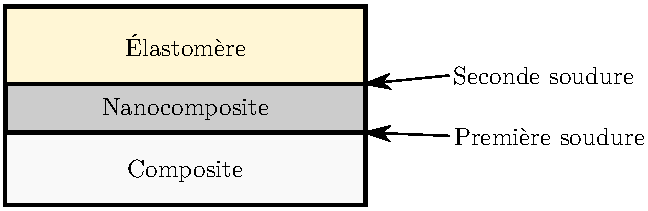
\includegraphics[scale=1]{jonction_multi_materiau.pdf}
	\caption{Schéma de la jonction multimatériaux présentant les deux soudures}
	\label{fig:scema_double_jonction}
\end{figure}

Aucun exemple d'un type de soudure similaire n'a pu être répertorié lors de la revue de la littérature. 
Ainsi, en raison de la nature exploratoire de cette portion du projet, les travaux de caractérisation sont réalisés avec une approche progressive et méthodique. 

\section{Méthodologie}

La première caractéristique à valider avant de réaliser le soudage est la stabilité thermique de l'élastomère. 
Il est nécessaire de vérifier que ce dernier pourra résister aux températures rencontrées lors du soudage sans se dégrader. 
Par la suite, des essais de caractérisation mécanique viennent valider les propriétés mécaniques de l'élastomère, ce dernier devant rencontrer les requis du cahier des charges. 
En parallèle à la caractérisation mécanique, des essais progressifs de soudage sont mis en œuvre pour valider la possibilité de souder le matériau choisi. 

\subsection{Matériaux}

L'élastomère retenu est un copolymère multiblocs (Fig. \ref{fig:polymere_multi_bloc}) de PEI et de polysiloxane  produit par SABIC sous le nom commercial ULTEM STM1500 avec des segments successifs de longueur variables  \cite{mark2013,Holden2002}. 
Il est à noter que la nature exacte de la structure du PEI-siloxane est matière à caution. 
Hatui présente la structure comme un simple copolymère alterné (Fig. \ref{fig:polymere_alternee}) \cite{Hatui2015}. 
Toujours selon cet auteur, le PEI-siloxane serait miscible avec le PEI. 

Les éléments chauffants ainsi que les adhérents en composite ont la même composition et ont été produits selon la même méthode que dans les chapitres \ref{sec:Theme1} et \ref{sec:Theme2}. 

\subsection{Caractérisation de la stabilité thermique des élastomères et du nanocomposite}

Des analyses thermogravimétriques (TGA) de l'élastomère ont été réalisées avec un appareil TA Instruments Q500. 
Tel qu'il est présenté dans la norme ASTM E2550 - 17, les échantillons ont été soumis à une rampe de \SI[locale=FR]{10}{\celsius\per\minute} jusqu'à une température de \SI[locale=FR]{800}{\celsius} sous une atmosphère régulière. 

Une seconde méthode plus sensible a été employée pour évaluer la stabilité thermique de l'élastomère. 
Les essais de TGA permettent de détecter la présence de dégradation lorsque la masse de l'échantillon change. 
Cependant, lorsque la dégradation se produit par une modification de la structure du polymère, par scission de chaines ou par réaction entre celles-ci, une mesure de la masse peut être insensible à ce changement. 
Ainsi, une mesure indirecte de la viscosité durant un brassage à haute température a pu être réalisée pour certains matériaux en suivant l'évolution temporelle du couple lors de la production d'un mélange en condition isotherme, et ce, à l'aide d'un mélangeur interne Haake PolyLab OS. 
Cette mesure permet d'identifier le début d'un processus de dégradation de l'élastomère. 
Une méthode permettant de quantifier la dégradation serait de mesurer l'évolution de la masse moléculaire ($M_n$ et $M_w$) du polymère avant le mélange et à divers moments du mélange. 

\subsection{Caractérisation mécanique des élastomères}

Les propriétés mécaniques des élastomères sont validées à l'aide d'essais de traction. 
Les essais de traction ont été effectués avec un échantillon de type V selon la norme ASTM~D638-14. 
Une plaque de \SI[locale=FR]{3.2}{\milli\metre} d'épaisseur a été produite par compression à chaud de granules. 
Les échantillons ont ensuite été découpés à l'aide d'un poinçon et d'une presse. 

\subsection{Essais de soudage}

Les essais de soudage sont réalisés en étapes afin de maximiser la possibilité d'obtenir une diffusion des chaines de polymères. 
Les premiers essais de soudage sont effectués sous vide dans une étuve chauffante (Fig. \ref{fig:schema_soudure_etuve}). 
Lors de ce test, un empilement d'échantillons de composite, de nanocomposite et d'élastomère est positionné dans l'étuve. 
Des poids sont ensuite ajoutés pour simuler la pression exercée lors du soudage. 
En raison de la taille de l'étuve et de l'échantillon ainsi que des poids disponibles, il a été impossible de maintenir en équilibre suffisamment de poids pour obtenir la même pression que dans le montage de soudage. 
L'échantillon est installé dans l'étuve avant le début du chauffage jusqu'à la température désirée. 

\begin{figure}[h]
	\centering
	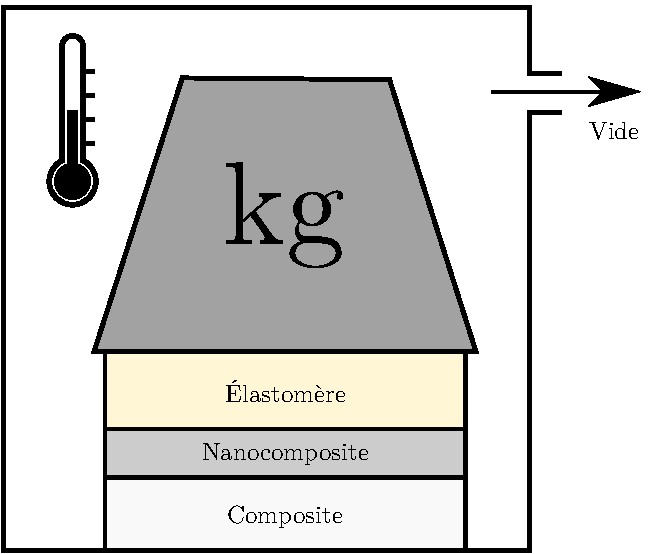
\includegraphics[scale=0.6]{schema_soudure_etuve.pdf}
	\caption{Schéma du procédé de soudage dans une étuve}
	\label{fig:schema_soudure_etuve}
\end{figure}

La seconde méthode utilisée est un soudage dans une presse chauffante manuelle (Fig. \ref{fig:schema_soudure_presse}). 
Durant ce test, un empilement symétrique en sandwich avec deux échantillons de composite et de nanocomposite ainsi qu'un échantillon d'élastomère au centre est positionné entre deux plaques métalliques. 
La presse est préchauffée à la température désirée avant d'insérer l'empilement. 
Lorsque les plateaux de la presse atteignent la température de consigne, une pression est appliquée sur l'empilement pour le consolider. 
Après 10 minutes, le chauffage de la presse est arrêté et un ventilateur est utilisé pour accélérer le refroidissement du montage. 
Les échantillons sont retirés de la presse une fois qu'ils sont refroidis. 

\begin{figure}[h]
	\centering
	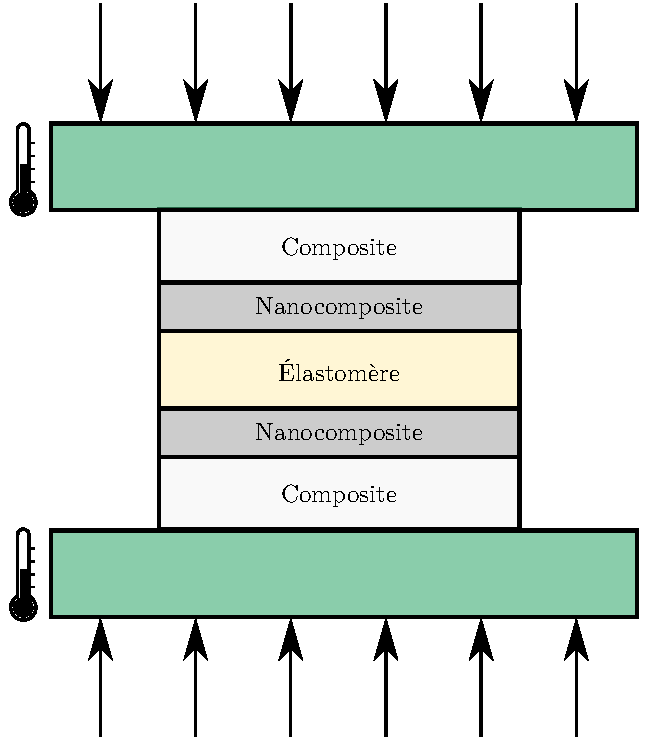
\includegraphics[scale=0.6]{schema_soudure_presse.pdf}
	\caption{Schéma du procédé de soudage à la presse chauffante}
	\label{fig:schema_soudure_presse}
\end{figure}

À la suite des premiers résultats, la possibilité de souder l'élastomère a été évaluée à l'aide du montage de soudage. 
Dans ce dernier, une couche d'élastomère est déposée sur un élément chauffant nanocomposite reposant sur un adhérent en composite. 
L'empilement était déposé sur une céramique isolante avant qu'un autre morceau de céramique ne soit positionné au-dessus de la soudure. 
Les vérins étaient ensuite abaissés pour appliquer une pression sur la zone soudée ainsi que sur les électrodes en contact avec le nanocomposite. 
La quantité de courant et le voltage appliqués durant les essais de soudage ont été contrôlés afin de maintenir une puissance électrique surfacique constante tout au long de chaque test. 

Deux modes de soudures distincts ont été évalués (Fig. \ref{fig:schema_processus_soudure_resistance}). 
\begin{enumerate}
	\item Produire les soudures des deux côtés de l'élément chauffant nanocomposite en une seule étape. 
	Ces essais visaient à produire une soudure multimatériaux complète entre le composite et le nanocomposite ainsi qu'entre l'élastomère et le nanocomposite en une seule étape. 
	\item Produire les soudures en deux étapes. 
	Une première soudure est produite entre le composite et le nanocomposite. 
	Une seconde soudure entre le nanocomposite et l'élastomère est ensuite produite en appliquant, de nouveau, un courant électrique dans le nanocomposite déjà soudé au composite. 
	Ce second mode de soudage avait pour but d'employer des conditions d'opération différentes pour chaque combinaison de matériau. 
\end{enumerate}

\begin{figure}[h]
	\centering
	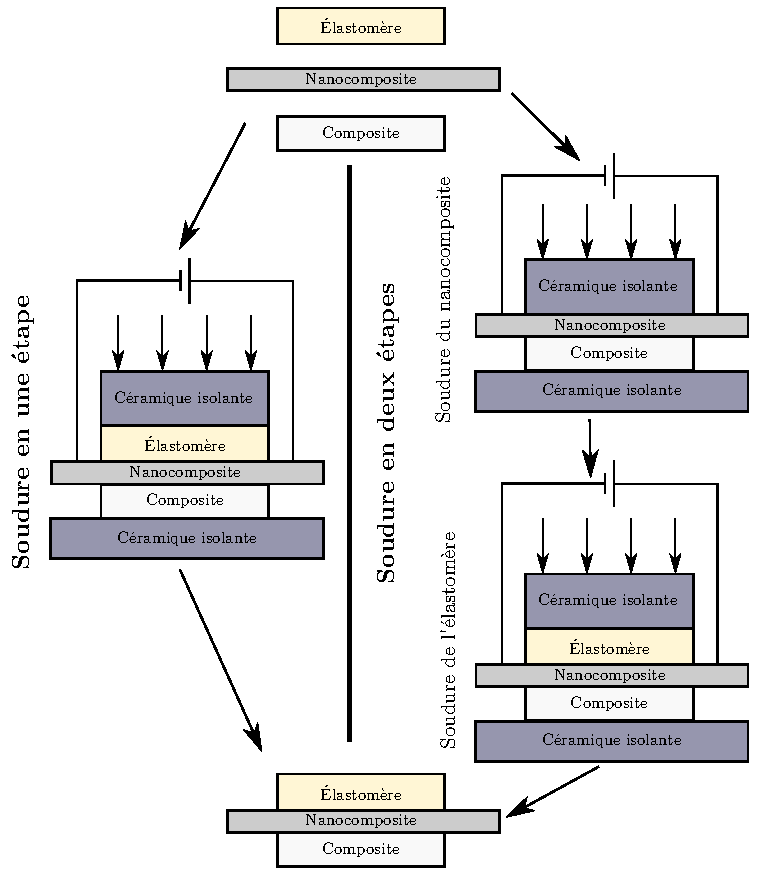
\includegraphics[scale=1]{schema_processus_soudure_resistance.pdf}
	\caption{Schéma du procédé de soudage par résistance montrant les processus en une étape et en deux étapes}
	\label{fig:schema_processus_soudure_resistance}
\end{figure}
\FloatBarrier

Lors du soudage des échantillons pour les essais de caractérisation mécanique, l'élément chauffant nanocomposite est positionné avec un retrait d'une distance d'environ 1 à \SI[locale=FR]{2}{\milli\metre} du bout de l'adhérent. 
L'élastomère est également positionné de façon à obtenir un retrait de 1 à \SI[locale=FR]{2}{\milli\metre} avec le bout de l'échantillon. 

\subsection{Caractérisation mécanique des joints soudés}

La résistance des soudures a été évaluée selon leur géométrie. 
Les essais dans l'étuve ou sous presse n'avaient pas une géométrie propice à des essais de caractérisation mécanique. 
Dans ces cas particuliers, la soudure était évaluée par pelage manuel du joint. 
Si nécessaire, des outils étaient utilisés pour tenter de décoller les faciès en contact. 
Après la séparation des faciès, une observation visuelle des joints, parfois suivie d'une observation au microscope optique, permet de juger de la qualité du joint. 

\begin{figure}[h]
	\centering
	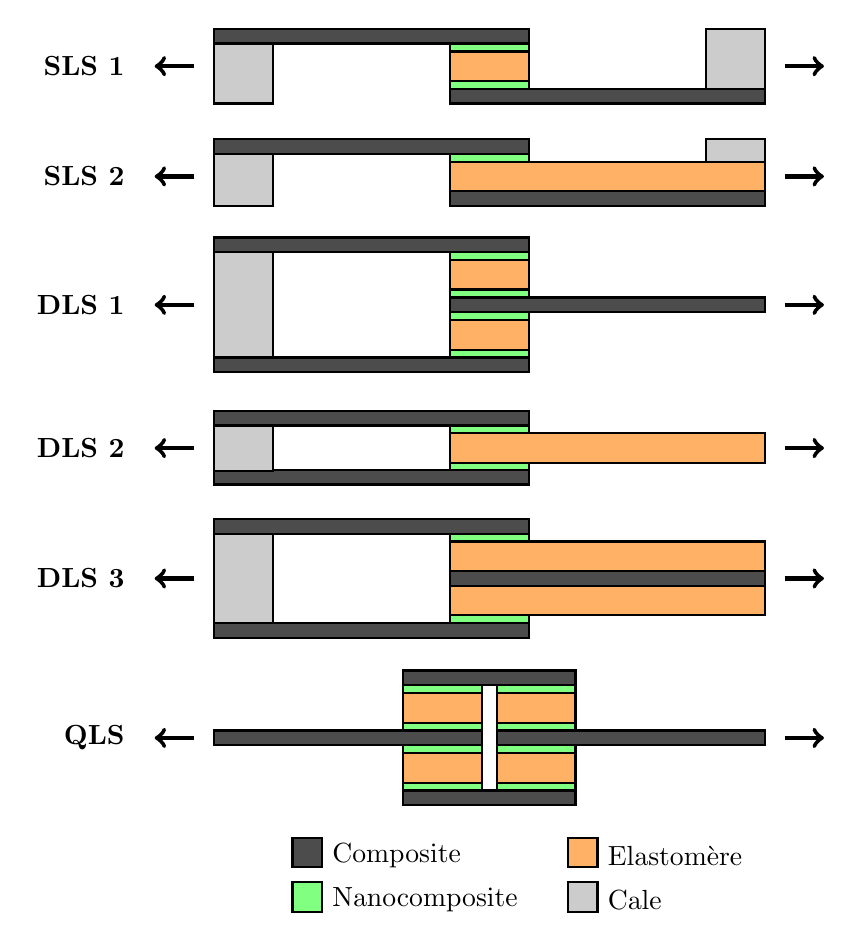
\begin{tikzpicture}[scale=0.5, thick]

%Dimensons générales
\def \overlap{2}
\def \espacevert{1}

%Dimensions composite
\def \lcomp{8}
\def \tcomp{0.375}

%Épaisseur de l'élément résistif
\def \tele{0.2}

%Épaisseur de l'élastomère
\def \tela{0.75}

%Dimensions de la calle
\def \lcalle{1.5}

%Position et taille des annotations
\def \lforce{1}
\def \gapforce{0.5}
\def \gaptexte{0.375}
\def \legende{0.75}
\def \gapscie{0.375}
\def \midgap{0.375}

%Couleurs
\def \colcomp{black!70}
\def \colele{green!50}
\def \colelas{orange!60}
\def \colcalle{black!20}


%\begin{scope}[shift={(0,21)}]
%	%Plaques
%	\draw[black,fill=\colcomp] (0,0) -- ++(0,\tcomp) -- ++(\lcomp,0) -- ++(0,-\tcomp) -- cycle; %Single shear haut
%	\draw[black,fill=\colcomp] (\lcomp-\overlap,-\tele-\tcomp) -- ++(0,\tcomp) -- ++(\lcomp,0) -- ++(0,-\tcomp) -- cycle; %Single shear bas
%	
%	%Éléments chauffants
%	\draw[black,fill=\colele] (\lcomp-\overlap,-\tele) -- ++(0,\tele) -- ++(\overlap,0) -- ++(0,-\tele) -- cycle; %Single shear
%	
%	%Calles
%	\draw[black,fill=\colcalle] (0,0) -- ++(0,-\tele-\tcomp) -- ++(\lcalle,0) -- ++(0,\tele+\tcomp) -- cycle; % calle 1
%	\draw[black,fill=\colcalle] (2*\lcomp-\overlap-\lcalle,\tcomp) -- ++(0,-\tele-\tcomp) -- ++(\lcalle,0) -- ++(0,\tele+\tcomp) -- cycle; % calle 2
%	
%	%Lignes de force
%	\begin{scope}[ultra thick]
%	\draw [->] (-\gapforce,-.5*\tele) -- ++(-\lforce,0);
%	\draw [->] (2*\lcomp-\overlap+\gapforce,-.5*\tele) -- ++(\lforce,0);
%	\end{scope}
%	
%	%Identification de l'éprouvette
%	\draw (-\lforce-2*\gapforce,-.5*\tele) node[left]{\textbf{SLS}};
%\end{scope}

\begin{scope}[shift={(0,18.8)}]
	%Plaques
	\draw[black,fill=\colcomp] (0,0) -- ++(0,\tcomp) -- ++(\lcomp,0) -- ++(0,-\tcomp) -- cycle; %single shear haut 1
	\draw[black,fill=\colcomp] (\lcomp-\overlap,-2*\tele-\tcomp-\tela) -- ++(0,\tcomp) -- ++(\lcomp,0) -- ++(0,-\tcomp) -- cycle; %single shear bas 2
	
	%Éléments chauffants
	\draw[black,fill=\colele] (\lcomp-\overlap,-\tele) -- ++(0,\tele) -- ++(\overlap,0) -- ++(0,-\tele) -- cycle; %single shear haut 2
	\draw[black,fill=\colele] (\lcomp-\overlap,-2*\tele-\tela) -- ++(0,\tele) -- ++(\overlap,0) -- ++(0,-\tele) -- cycle; %single shear bas 2
	
	%Élastomère
	\draw[black,fill=\colelas] (\lcomp-\overlap,-\tela-\tele) -- ++(0,\tela) -- ++(\overlap,0) -- ++(0,-\tela) -- cycle; % elastomère 2

	%Calles
	\draw[black,fill=\colcalle] (0,0) -- ++(0,-2*\tele-\tcomp-\tela) -- ++(\lcalle,0) -- ++(0,2*\tele+\tcomp+\tela) -- cycle; % calle 1
	\draw[black,fill=\colcalle] (2*\lcomp-\overlap-\lcalle,\tcomp) -- ++(0,-2*\tele-\tcomp-\tela) -- ++(\lcalle,0) -- ++(0,2*\tele+\tcomp+\tela) -- cycle; % calle 2
	
	%Lignes de force
	\begin{scope}[ultra thick]
	\draw [->] (-\gapforce,-\tele-0.5*\tela) -- ++(-\lforce,0);
	\draw [->] (2*\lcomp-\overlap+\gapforce,-\tele-0.5*\tela) -- ++(\lforce,0);
	\end{scope}
	
	%Identification de l'éprouvette
	\draw (-\lforce-2*\gapforce,-\tele-0.5*\tela) node[left]{\textbf{SLS 1}};
\end{scope}

\begin{scope}[shift={(0,16)}] 
	%Plaques
	\draw[black,fill=\colcomp] (0,0) -- ++(0,\tcomp) -- ++(\lcomp,0) -- ++(0,-\tcomp) -- cycle; %single shear haut 1
	\draw[black,fill=\colcomp] (\lcomp-\overlap,-\tele-\tcomp-\tela) -- ++(0,\tcomp) -- ++(\lcomp,0) -- ++(0,-\tcomp) -- cycle; %single shear bas 2
	
	%Éléments chauffants
	\draw[black,fill=\colele] (\lcomp-\overlap,-\tele) -- ++(0,\tele) -- ++(\overlap,0) -- ++(0,-\tele) -- cycle; %single shear haut 2

	%Élastomère
	\draw[black,fill=\colelas] (\lcomp-\overlap,-\tela-\tele) -- ++(0,\tela) -- ++(\lcomp,0) -- ++(0,-\tela) -- cycle; % elastomère 2

	%Calles
	\draw[black,fill=\colcalle] (0,0) -- ++(0,-\tele-\tcomp-\tela) -- ++(\lcalle,0) -- ++(0,\tele+\tcomp+\tela) -- cycle; % calle 1
	\draw[black,fill=\colcalle] (2*\lcomp-\overlap-\lcalle,\tcomp) -- ++(0,-\tele-\tcomp) -- ++(\lcalle,0) -- ++(0,\tele+\tcomp) -- cycle; % calle 2
	
	%Lignes de force
	\begin{scope}[ultra thick]
	\draw [->] (-\gapforce,-\tele-0.5*\tela) -- ++(-\lforce,0);
	\draw [->] (2*\lcomp-\overlap+\gapforce,-\tele-0.5*\tela) -- ++(\lforce,0);
	\end{scope}
	
	%Identification de l'éprouvette
	\draw (-\lforce-2*\gapforce,-\tele-0.5*\tela) node[left]{\textbf{SLS 2}};
\end{scope}


\begin{scope}[shift={(0,13.5)}]
	%Plaques
	\draw[black,fill=\colcomp] (0,0) -- ++(0,\tcomp) -- ++(\lcomp,0) -- ++(0,-\tcomp) -- cycle; %dual shear haut
	\draw[black,fill=\colcomp] (\lcomp-\overlap,-2*\tele-\tcomp-\tela) -- ++(0,\tcomp) -- ++(\lcomp,0) -- ++(0,-\tcomp) -- cycle; %dual shear milieu
	\draw[black,fill=\colcomp] (0,-2*\tcomp-4*\tele-2*\tela) -- ++(0,\tcomp) -- ++(\lcomp,0) -- ++(0,-\tcomp) -- cycle; %dual shear bas
	
	%Éléments chauffants
	\draw[black,fill=\colele] (\lcomp-\overlap,-\tele) -- ++(0,\tele) -- ++(\overlap,0) -- ++(0,-\tele) -- cycle; %dual shear haut 1
	\draw[black,fill=\colele] (\lcomp-\overlap,-2*\tele-\tela) -- ++(0,\tele) -- ++(\overlap,0) -- ++(0,-\tele) -- cycle; %dual shear haut 2
	\draw[black,fill=\colele] (\lcomp-\overlap,-3*\tele-\tela-\tcomp) -- ++(0,\tele) -- ++(\overlap,0) -- ++(0,-\tele) -- cycle; %dual shear bas 1
	\draw[black,fill=\colele] (\lcomp-\overlap,-4*\tele-2*\tela-\tcomp) -- ++(0,\tele) -- ++(\overlap,0) -- ++(0,-\tele) -- cycle; %dual shear bas 2
	
	%Élastomère
	\draw[black,fill=\colelas] (\lcomp-\overlap,-\tela-\tele) -- ++(0,\tela) -- ++(\overlap,0) -- ++(0,-\tela) -- cycle; % elastomère haut
	\draw[black,fill=\colelas] (\lcomp-\overlap,-2*\tela-3*\tele-\tcomp) -- ++(0,\tela) -- ++(\overlap,0) -- ++(0,-\tela) -- cycle; % elastomère bas
	
	%Calle
	\draw[black,fill=\colcalle] (0,0) -- ++(0,-4*\tele-2*\tela-\tcomp) -- ++(\lcalle,0) -- ++(0,4*\tele+2*\tela+\tcomp) -- cycle; % calle
	
	%Lignes de force
	\begin{scope}[ultra thick]
	\draw [->] (-\gapforce,-2*\tele-\tela-0.5*\tcomp) -- ++(-\lforce,0);
	\draw [->] (2*\lcomp-\overlap+\gapforce,-2*\tele-\tela-0.5*\tcomp) -- ++(\lforce,0);
	\end{scope}
	
	%Identification de l'éprouvette
	\draw (-\lforce-2*\gapforce,-2*\tele-\tela-0.5*\tcomp) node[left]{\textbf{DLS 1}};
\end{scope}


\begin{scope}[shift={(0,9.1)}] 
	%Plaques
	\draw[black,fill=\colcomp] (0,0) -- ++(0,\tcomp) -- ++(\lcomp,0) -- ++(0,-\tcomp) -- cycle; %dual shear haut
	\draw[black,fill=\colcomp] (0,-2*\tcomp-\tela) -- ++(0,\tcomp) -- ++(\lcomp,0) -- ++(0,-\tcomp) -- cycle; %dual shear bas
	
	%Éléments chauffants
	\draw[black,fill=\colele] (\lcomp-\overlap,-\tele) -- ++(0,\tele) -- ++(\overlap,0) -- ++(0,-\tele) -- cycle; %dual shear haut 1
	\draw[black,fill=\colele] (\lcomp-\overlap,-\tela-\tcomp) -- ++(0,\tele) -- ++(\overlap,0) -- ++(0,-\tele) -- cycle; %dual shear bas 2
	
	%Élastomère
	\draw[black,fill=\colelas] (\lcomp-\overlap,-\tela-\tele) -- ++(0,\tela) -- ++(\lcomp,0) -- ++(0,-\tela) -- cycle; % elastomère haut
	
	%Calle
	\draw[black,fill=\colcalle] (0,0) -- ++(0,-2*\tele-\tela) -- ++(\lcalle,0) -- ++(0,2*\tele+\tela) -- cycle; % calle
	
	%Lignes de force
	\begin{scope}[ultra thick]
	\draw [->] (-\gapforce,-\tele-0.5*\tela) -- ++(-\lforce,0);
	\draw [->] (2*\lcomp-\overlap+\gapforce,-\tele-0.5*\tela) -- ++(\lforce,0);
	\end{scope}
	
	%Identification de l'éprouvette
	\draw (-\lforce-2*\gapforce,-\tele-0.5*\tela) node[left]{\textbf{DLS 2}};
\end{scope}


\begin{scope}[shift={(0,6.35)}] 
	%Plaques
	\draw[black,fill=\colcomp] (0,0) -- ++(0,\tcomp) -- ++(\lcomp,0) -- ++(0,-\tcomp) -- cycle; %dual shear haut
	\draw[black,fill=\colcomp] (\lcomp-\overlap,-\tele-\tcomp-\tela) -- ++(0,\tcomp) -- ++(\lcomp,0) -- ++(0,-\tcomp) -- cycle; %dual shear milieu
	\draw[black,fill=\colcomp] (0,-2*\tcomp-2*\tele-2*\tela) -- ++(0,\tcomp) -- ++(\lcomp,0) -- ++(0,-\tcomp) -- cycle; %dual shear bas
	
	%Éléments chauffants
	\draw[black,fill=\colele] (\lcomp-\overlap,-\tele) -- ++(0,\tele) -- ++(\overlap,0) -- ++(0,-\tele) -- cycle; %dual shear haut 1
	\draw[black,fill=\colele] (\lcomp-\overlap,-2*\tele-2*\tela-\tcomp) -- ++(0,\tele) -- ++(\overlap,0) -- ++(0,-\tele) -- cycle; %dual shear bas 2
	
	%Élastomère
	\draw[black,fill=\colelas] (\lcomp-\overlap,-\tela-\tele) -- ++(0,\tela) -- ++(\lcomp,0) -- ++(0,-\tela) -- cycle; % elastomère haut
	\draw[black,fill=\colelas] (\lcomp-\overlap,-2*\tela-1*\tele-\tcomp) -- ++(0,\tela) -- ++(\lcomp,0) -- ++(0,-\tela) -- cycle; % elastomère bas
	
	%Calle
	\draw[black,fill=\colcalle] (0,0) -- ++(0,-2*\tele-2*\tela-\tcomp) -- ++(\lcalle,0) -- ++(0,2*\tele+2*\tela+\tcomp) -- cycle; % calle
	
	%Lignes de force
	\begin{scope}[ultra thick]
	\draw [->] (-\gapforce,-\tele-\tela-0.5*\tcomp) -- ++(-\lforce,0);
	\draw [->] (2*\lcomp-\overlap+\gapforce,-\tele-\tela-0.5*\tcomp) -- ++(\lforce,0);
	\end{scope}
	
	%Identification de l'éprouvette
	\draw (-\lforce-2*\gapforce,-\tele-\tela-0.5*\tcomp) node[left]{\textbf{DLS 3}};
\end{scope}


\begin{scope}[shift={(0,2.5)}]
	%Plaques
	\draw[black,fill=\colcomp] (\lcomp-1.5*\overlap-0.5*\midgap,0) -- ++(0,\tcomp) -- ++(2*\overlap+\midgap,0) -- ++(0,-\tcomp) -- cycle; %quad shear haut
	\draw[black,fill=\colcomp] (0,-2*\tele-\tcomp-\tela) -- ++(0,\tcomp) -- ++(\lcomp-0.5*\overlap-0.5*\midgap,0) -- ++(0,-\tcomp) -- cycle; %quad shear milieu 1
	\draw[black,fill=\colcomp] (\lcomp-0.5*\overlap+0.5*\midgap,-2*\tele-\tcomp-\tela) -- ++(0,\tcomp) -- ++(\lcomp-0.5*\overlap-0.5*\midgap,0) -- ++(0,-\tcomp) -- cycle; %quad shear milieu 2
	\draw[black,fill=\colcomp] (\lcomp-1.5*\overlap-0.5*\midgap,-2*\tcomp-4*\tele-2*\tela) -- ++(0,\tcomp) -- ++(2*\overlap+\midgap,0) -- ++(0,-\tcomp) -- cycle; %quad shear bas
	
	%Éléments chauffants 
	
	%gauche
	\draw[black,fill=\colele] (\lcomp-1.5*\overlap-0.5*\midgap,-\tele) -- ++(0,\tele) -- ++(\overlap,0) -- ++(0,-\tele) -- cycle; %quad shear haut 1
	\draw[black,fill=\colele] (\lcomp-1.5*\overlap-0.5*\midgap,-2*\tele-\tela) -- ++(0,\tele) -- ++(\overlap,0) -- ++(0,-\tele) -- cycle; %quad shear haut 2
	\draw[black,fill=\colele] (\lcomp-1.5*\overlap-0.5*\midgap,-3*\tele-\tela-\tcomp) -- ++(0,\tele) -- ++(\overlap,0) -- ++(0,-\tele) -- cycle; %quad shear bas 1
	\draw[black,fill=\colele] (\lcomp-1.5*\overlap-0.5*\midgap,-4*\tele-2*\tela-\tcomp) -- ++(0,\tele) -- ++(\overlap,0) -- ++(0,-\tele) -- cycle; %quad shear bas 2
	
	%droite
	\draw[black,fill=\colele] (\lcomp-0.5*\overlap+0.5*\midgap,-\tele) -- ++(0,\tele) -- ++(\overlap,0) -- ++(0,-\tele) -- cycle; %quad shear haut 1
	\draw[black,fill=\colele] (\lcomp-0.5*\overlap+0.5*\midgap,-2*\tele-\tela) -- ++(0,\tele) -- ++(\overlap,0) -- ++(0,-\tele) -- cycle; %quad shear haut 2
	\draw[black,fill=\colele] (\lcomp-0.5*\overlap+0.5*\midgap,-3*\tele-\tela-\tcomp) -- ++(0,\tele) -- ++(\overlap,0) -- ++(0,-\tele) -- cycle; %quad shear bas 1
	\draw[black,fill=\colele] (\lcomp-0.5*\overlap+0.5*\midgap,-4*\tele-2*\tela-\tcomp) -- ++(0,\tele) -- ++(\overlap,0) -- ++(0,-\tele) -- cycle; %quad shear bas 2
	
	%Élastomère
	
	%gauche
	\draw[black,fill=\colelas] (\lcomp-1.5*\overlap-0.5*\midgap,-\tela-\tele) -- ++(0,\tela) -- ++(\overlap,0) -- ++(0,-\tela) -- cycle; % elastomère haut 1
	\draw[black,fill=\colelas] (\lcomp-1.5*\overlap-0.5*\midgap,-2*\tela-3*\tele-\tcomp) -- ++(0,\tela) -- ++(\overlap,0) -- ++(0,-\tela) -- cycle; % elastomère bas 1
	
	%droite
	\draw[black,fill=\colelas] (\lcomp-0.5*\overlap+0.5*\midgap,-\tela-\tele) -- ++(0,\tela) -- ++(\overlap,0) -- ++(0,-\tela) -- cycle; % elastomère haut 1
	\draw[black,fill=\colelas] (\lcomp-0.5*\overlap+0.5*\midgap,-2*\tela-3*\tele-\tcomp) -- ++(0,\tela) -- ++(\overlap,0) -- ++(0,-\tela) -- cycle; % elastomère bas 1
	
	%Lignes de force
	\begin{scope}[ultra thick]
	\draw [->] (-\gapforce,-2*\tele-\tela-0.5*\tcomp) -- ++(-\lforce,0);
	\draw [->] (2*\lcomp-\overlap+\gapforce,-2*\tele-\tela-0.5*\tcomp) -- ++(\lforce,0);
	\end{scope}
	
	%Identification de l'éprouvette
	\draw (-\lforce-2*\gapforce,-2*\tele-\tela-0.5*\tcomp) node[left]{\textbf{QLS}};
\end{scope}

\begin{scope}[shift={(2,0)}]
	%Legende
	\draw [black, fill=\colcomp] (0,-\espacevert-1.5*\legende) rectangle ++(\legende,\legende);
	\draw (\legende,-\espacevert-\legende-.075) node[right]{Composite};

	\draw [black, fill=\colele] (0,-\espacevert-3*\legende) rectangle ++(\legende,\legende);
	\draw (\legende,-\espacevert-2.5*\legende-.075) node[right]{Nanocomposite};

	\draw [black, fill=\colelas] (7,-\espacevert-1.5*\legende) rectangle ++(\legende,\legende);
	\draw (7+\legende,-\espacevert-\legende-.075) node[right]{Elastomère};

	\draw [black, fill=\colcalle] (7,-\espacevert-3*\legende) rectangle ++(\legende,\legende);
	\draw (7+\legende,-\espacevert-2.5*\legende-.075) node[right]{Cale};

\end{scope}

\end{tikzpicture}

	\caption{Géométries en simple cisaillement (SLS), en double cisaillement (DLS) et en quadruple cisaillement (QLS) évaluées pour les essais de caractérisation mécanique de la jonction flexible}
	\label{fig:geometrie_echantillons}
\end{figure}
\FloatBarrier

Pour de déterminer la géométrie optimale des échantillons afin d'évaluer la résistance des joints soudés avec le montage de soudage par résistance, des modèles par éléments finis ont été développés. 
Plusieurs géométries d'échantillons comprenant des joints en simple cisaillement (SLS), des joints en double cisaillement (DLS) et des joints en quadruple cisaillement (QLS) ont été évaluées (Fig. \ref{fig:geometrie_echantillons}). 
Avant de procéder à la modélisation, une analyse des capacités de production a déterminé que les joints évalués devraient autant que possible n'avoir qu'une seule soudure. 
Également, la solution retenue devait limiter la déformation en rotation du joint causée par l'épaisseur de l'élastomère. 

Il a été jugé que les géométries DSL 1 et QLS n'étaient pas des solutions désirables en raison du nombre de soudures à réaliser. 
De plus, la solution SLS 1, nécessitant 2 soudures et causant une déformation en rotation du joint, ne présentait aucun avantage par rapport à la solution SLS 2 qui ne nécessite qu'une seule soudure. 

Des modèles par éléments finis ont été établis pour les solutions SLS 2, DLS 2 et DLS 3 dans le logiciel COMSOL Mul\-ti\-phy\-sics\-\textregistered . 
Dans ces modèles, basés sur les propriétés des matériaux, une force était appliquée de façon à simuler un essai mécanique en simple ou en double cisaillement avec des échantillons fixés dans les mors d'une machine de traction. 
L'extrémité d'un des adhérents était fixée et l'extrémité de l'autre était soumise à un chargement dans l'axe de l'échantillon sans possibilité de se déplacer ou de se déformer dans une autre direction. 

\begin{figure}[h]
	\centering
	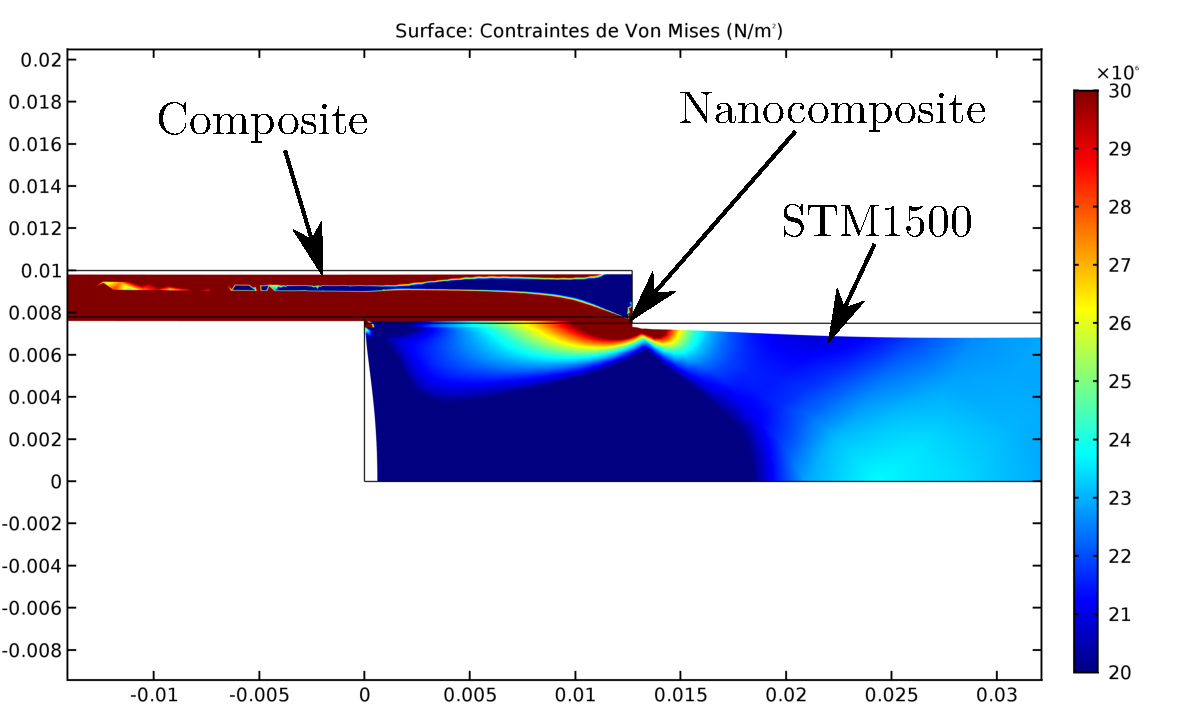
\includegraphics[width=0.6\textwidth]{DLS_Comp-TPE.pdf}
	\caption{Déformations et champ de contrainte pour un échantillon DLS 2 avec une couche d'élastomère de \SI[locale=FR]{15}{\milli\metre} d'épaisseur. Un plan de symétrie au milieu de l'élastomère est employé pour simplifier le modèle.}
	\label{fig:DLS_comp_TPE}
\end{figure}
\FloatBarrier

L'analyse des résultats pour la solution DSL 2 (Fig. \ref{fig:DLS_comp_TPE}), avec une couche d'élastomère servant d'adhérent, a démontré que la fabrication de cet échantillon nécessiterait un adhérent élastomère avec une épaisseur d'au moins \SI[locale=FR]{15}{\milli\metre} afin d'obtenir une rupture dans le joint plutôt qu'une rupture en tension de l'adhérent. 
Cette analyse ne prend pas en compte l'effet local des mâchoires. 
Une rupture pourrait se produire dans cette zone. 
Le tout est sans compter la difficulté de produire un échantillon de \SI[locale=FR]{15}{\milli\metre} d'épaisseur sans défauts. 
À la lumière de ces résultats, la géométrie d'échantillon DSL 2 a été mise de côté.

\begin{figure}[h!]
	\centering
	\subfigure[]
	{\label{fig:DLS_metal_1mm} 								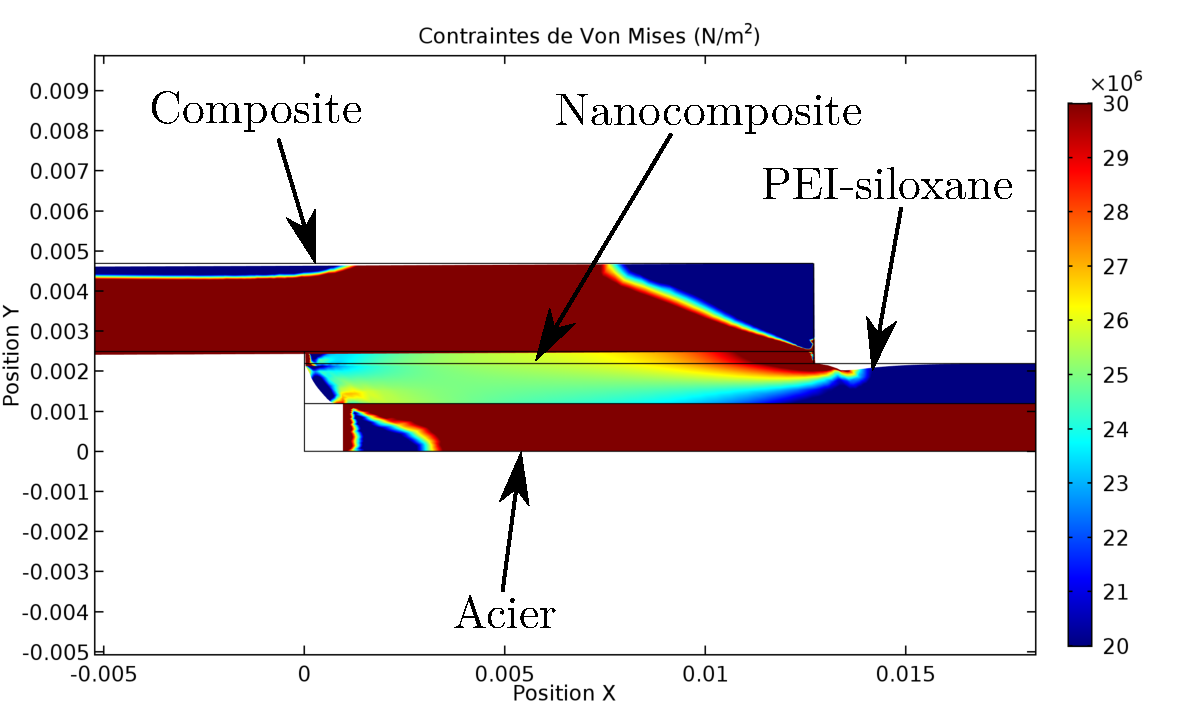
\includegraphics[width=0.6\textwidth]{DLS_Comp-TPE(metal)_1mm.pdf}
	} \\
	\subfigure[]
	{\label{fig:DLS_metal_2mm}
		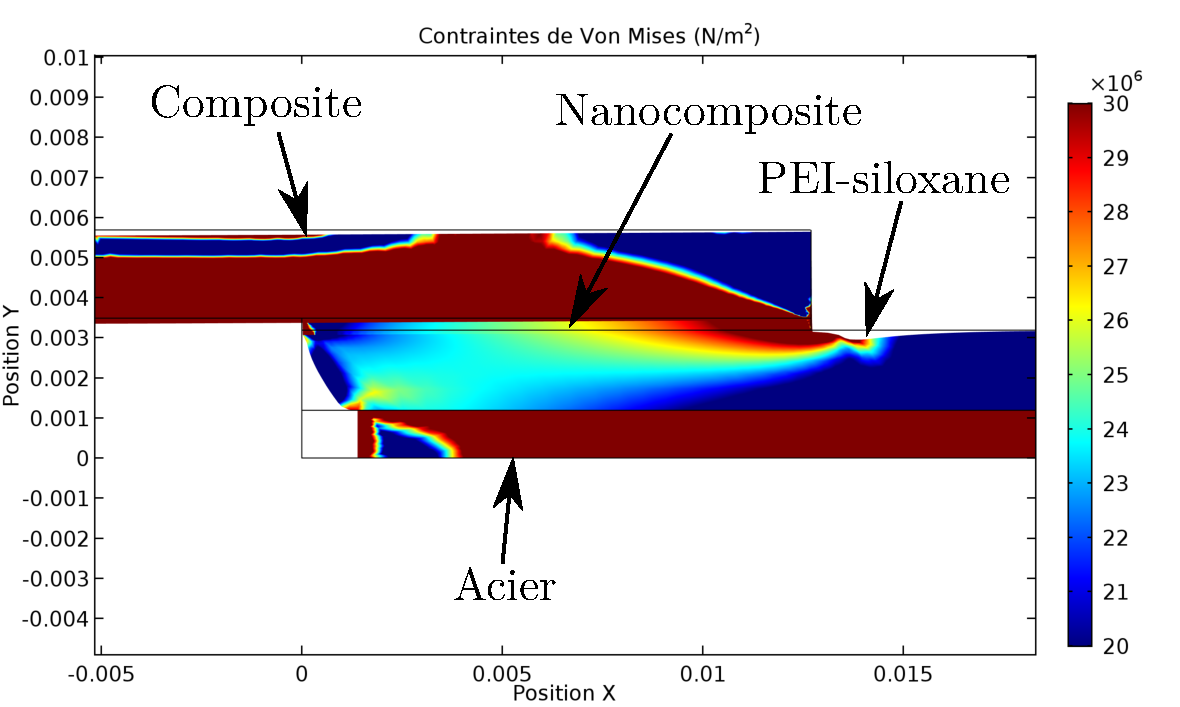
\includegraphics[width=0.6\textwidth]{DLS_Comp-TPE(metal)_2mm.pdf}
	} \\
	\subfigure[]
	{\label{fig:DLS_metal_5mm}
		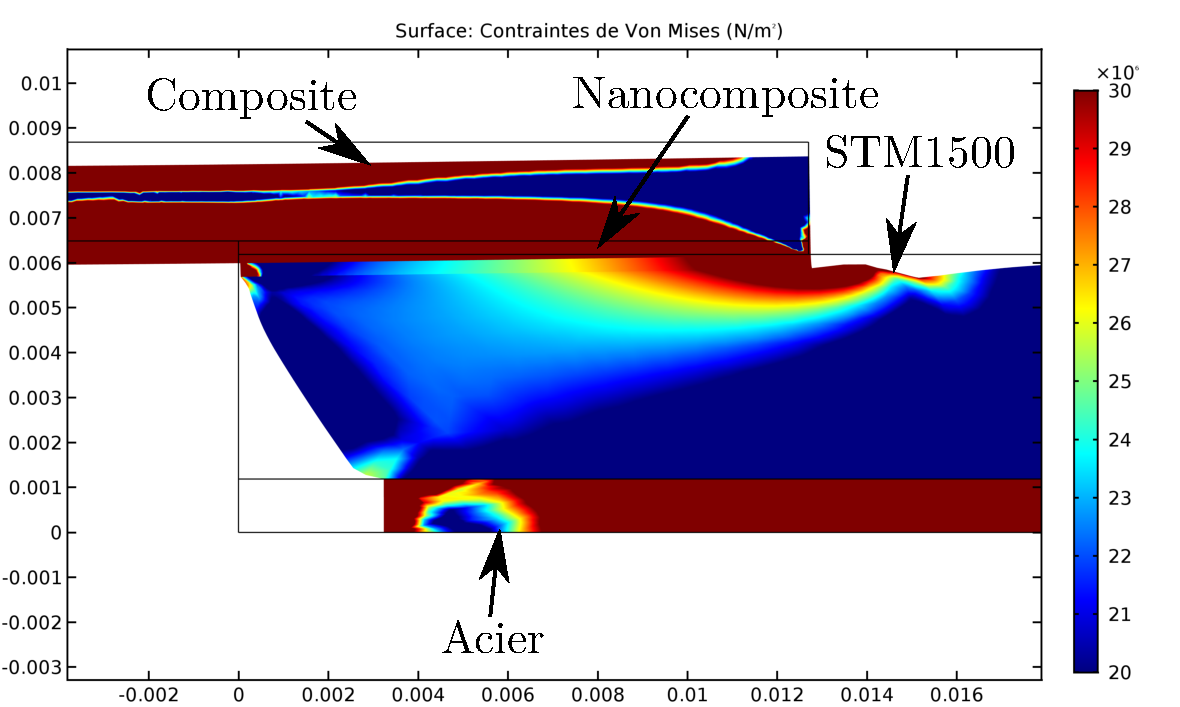
\includegraphics[width=0.6\textwidth]{DLS_Comp-TPE(metal)_5mm.pdf}
	}
	\caption{Analyse de l'effet de l'épaisseur de l'élastomère sur le champ de contrainte dans les échantillons DLS 3, avec un substrat en acier. Un plan de symétrie au milieu du substrat en acier est employé pour simplifier le modèle. Champs de contrainte pour des épaisseurs d'élastomère de a) \SI{1}{\milli\metre}, b) \SI{2}{\milli\metre} et c) \SI{5}{\milli\metre}}
	\label{fig:DLS_metal}
\end{figure}

Les prochains modèles ont étudié la géométrie DSL 3 où des couches d'élastomère sont collées sur un substrat en composite ou en acier (Fig. \ref{fig:DLS_metal}). 
Cette géométrie avait pour but de limiter le transfert de charge au travers de l'élastomère. 
Le principal élément évalué avec ces simulations est l'effet de l'épaisseur de l'élastomère sur le champ de contrainte. 
Il est important d'éviter les effets de bord causés par le substrat rigide lorsqu'une couche d'élastomère trop mince est utilisée. 
On peut voir qu'une épaisseur d'élastomère de \SI[locale=FR]{1}{\milli\metre} (Fig. \ref{fig:DLS_metal_1mm}) produit un champ de contrainte qui est fortement affecté par la présence d'un substrat en acier. 
Lorsque l'épaisseur de l'élastomère est augmentée à 2 et \SI[locale=FR]{5}{\milli\metre} (Fig. \ref{fig:DLS_metal_2mm} et \ref{fig:DLS_metal_5mm}), le champ de contrainte est de moins en moins affecté par l'influence du substrat. 
Une épaisseur supérieure à \SI[locale=FR]{2}{\milli\metre} est alors suffisante pour minimiser l'effet du substrat en acier sur la jonction soudée. 

\begin{figure}[h]
	\centering
	\subfigure[]
	{\label{fig:SLS_metal_1mm} 								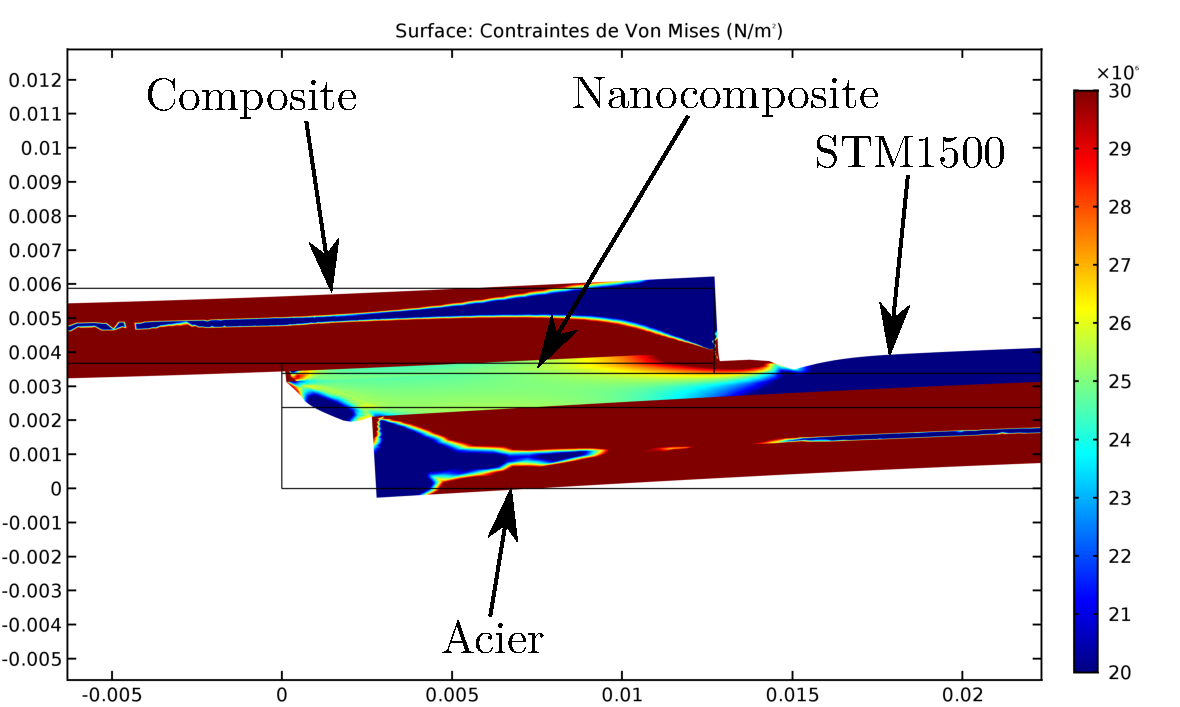
\includegraphics[width=0.6\textwidth]{SLS_Comp-TPE(metal)_1mm.pdf}
	}\qquad
	\subfigure[]
	{\label{fig:SLS_metal_2mm}
		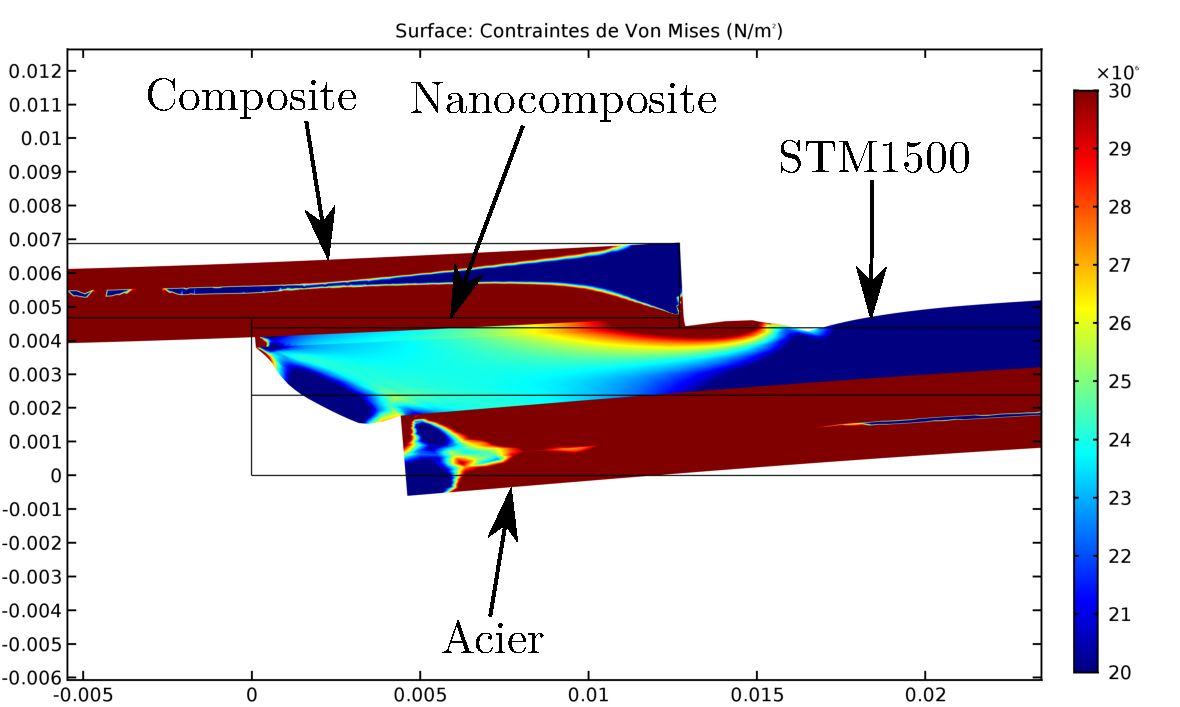
\includegraphics[width=0.6\textwidth]{SLS_Comp-TPE(metal)_2mm.pdf}
	} 
	\subfigure[]
	{\label{fig:SLS_metal_5mm}
		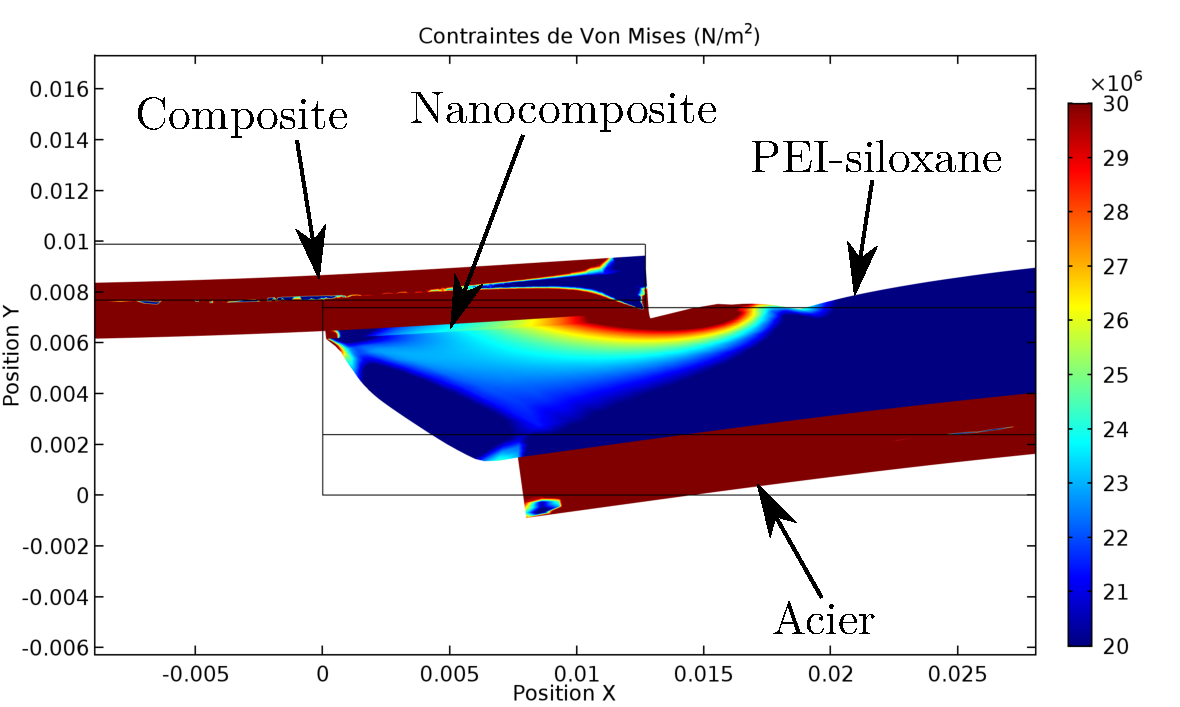
\includegraphics[width=0.6\textwidth]{SLS_Comp-TPE(metal)_5mm.pdf}
	} 
	\caption{Analyse de la rotation et du champ de contrainte dans les échantillons SLS 2, avec un substrat en acier. Champs de contrainte pour des épaisseurs d'élastomère de a) \SI{1}{\milli\metre}, b)~\SI{2}{\milli\metre} et c) \SI{5}{\milli\metre}}
	\label{fig:SLS_metal}
\end{figure}

Afin d'évaluer la possibilité d'utiliser une géométrie plus simple à produire pour les échantillons, des modèles par éléments finis ont été développés pour analyser la rotation du joint et le champ de contrainte dans l'élastomère pour la géométrie SLS 2 (Fig. \ref{fig:SLS_metal}). 
Un autre but de ce modèle était de déterminer l'épaisseur requise pour le substrat en acier afin de minimiser les déformations hors du plan.  
Le premier constat lors de l'analyse des résultats est que l'épaisseur de l'élastomère a le même impact sur le champ de contrainte. 
L'évaluation de l'épaisseur nécessaire pour obtenir un champ de contrainte non affecté par le substrat en acier, précédemment effectuée pour la géométrie DLS 3, reste donc valide pour cette géométrie, soit lorsque le substrat en acier possède une rigidité suffisante pour minimiser la rotation du joint. 
Un deuxième constat est qu'une plaque d'acier de \SI[locale=FR]{2.4}{\milli\metre} d'épaisseur permet de minimiser la rotation du joint. 

Au vu de ces analyses, il a été décidé que la performance des joints produits avec le montage de soudage par résistance serait évaluée à l'aide d'un chargement en simple cisaillement entre deux adhérents selon la géométrie SLS 2. 
En raison des moules disponibles, une couche d'élastomère de \SI[locale=FR]{3.18}{\milli\metre} a été utilisée avec un substrat en acier de \SI[locale=FR]{2.4}{\milli\metre}. 
Les adhérents d'élastomère ont été collés aux substrats d'acier à l'aide d'une colle époxyde structurelle. 
Des talons ont été installés aux deux extrémités pour faciliter le montage de l'échantillon dans la machine de traction. 
Les essais de caractérisation mécanique ont été réalisés avec une machine Landmark de MTS qui possède une cellule de charge de \SI[locale=FR]{100}{\kilo\newton}. 

\FloatBarrier
\section{Résultats et analyse}

\subsection{Stabilité thermique du nanocomposite}

En parallèle des essais de caractérisation thermique de l'élastomère, la stabilité thermique du nanocomposite a été validée. 
Cette dernière étant en quelque sorte la limite opérationnelle du procédé de soudage, les élastomères ne devraient jamais être exposés à des températures aussi élevées. 
Comme prévu, le PEI du nanocomposite a démontré des signes de dégradation lorsque la température a dépassé \SI[locale=FR]{450}{\celsius} (Fig. \ref{fig:TGA_nanocomposite}). 

\begin{figure}[htb]
	\centering
	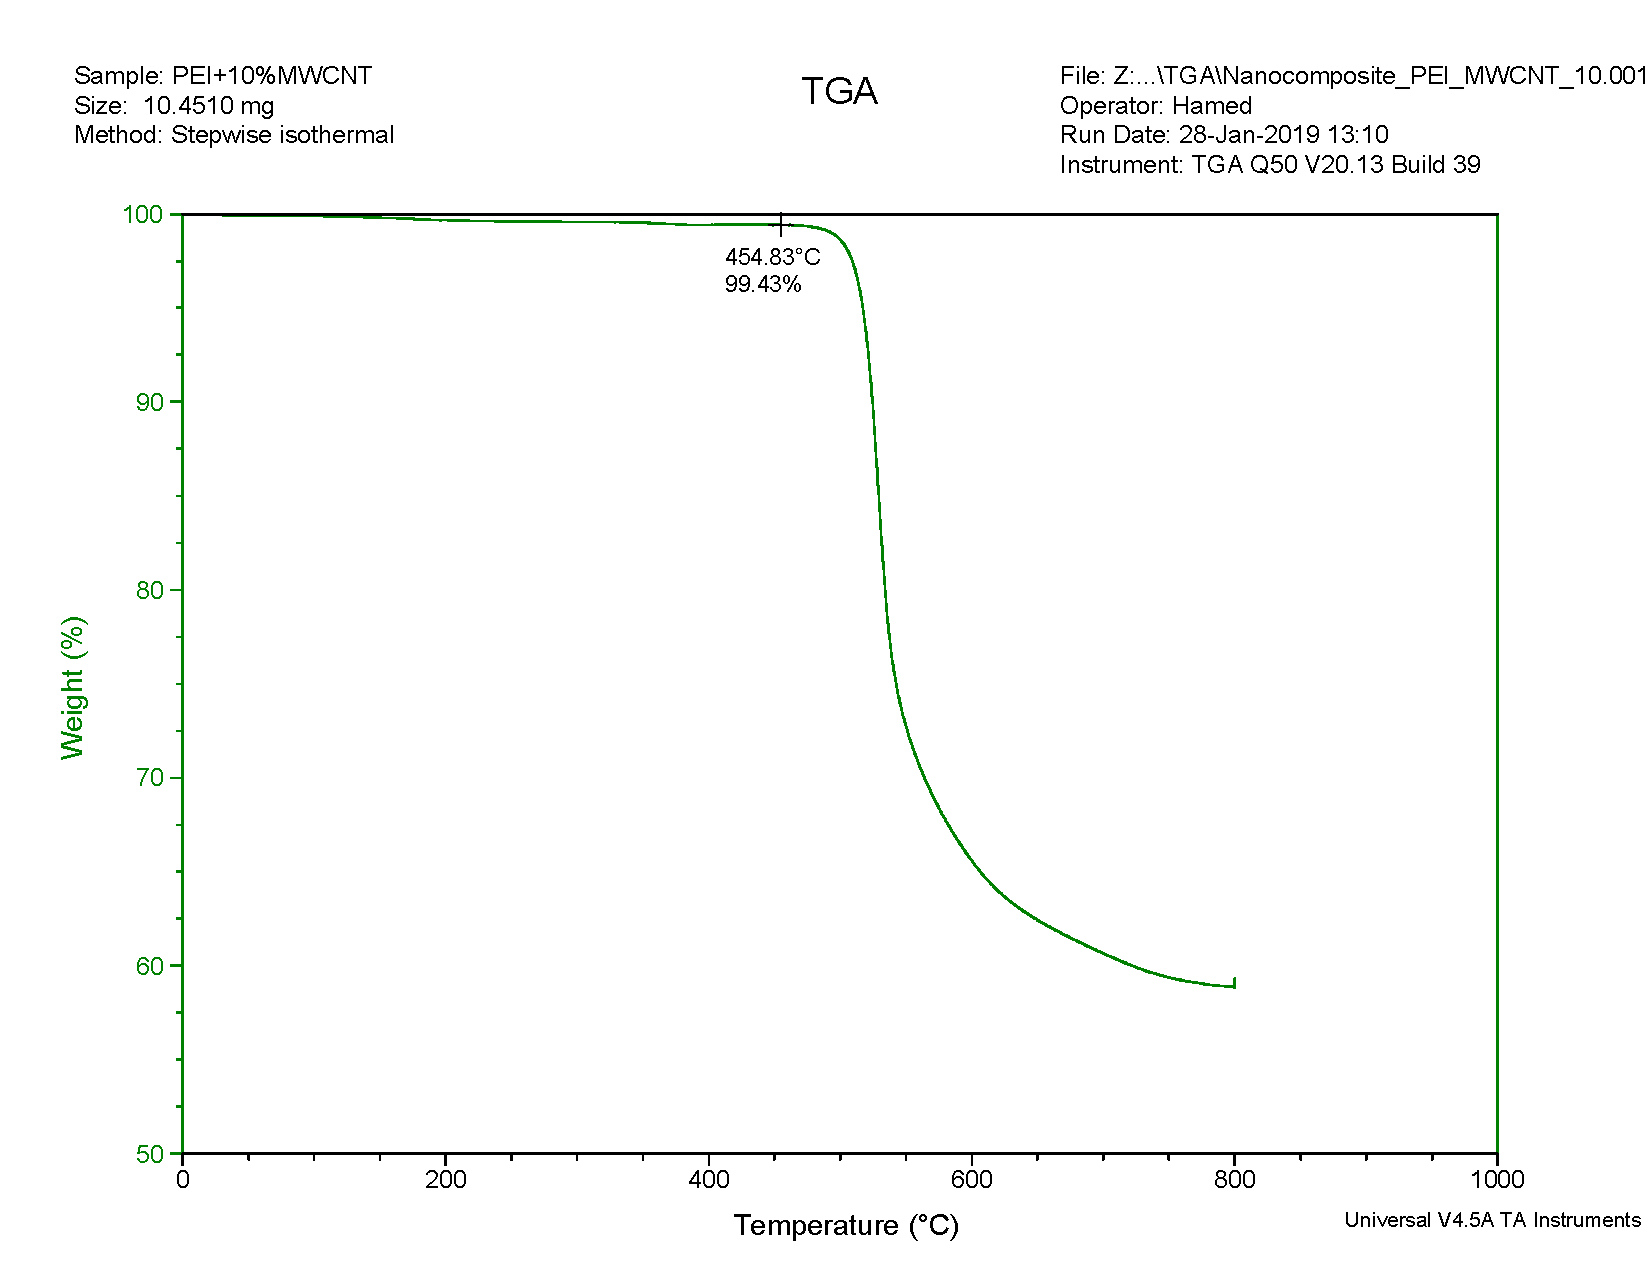
\includegraphics[width=0.95\textwidth]{TGA_nanocomposite.pdf}
	\caption{Résultats en TGA dans l'air pour le nanocomposite}
	\label{fig:TGA_nanocomposite}
\end{figure}

\FloatBarrier
\subsection{Stabilité thermique de l'élastomère}

La stabilité thermique du PEI-siloxane a été évaluée. 
L'élastomère a conservé au moins 99,5\% de sa masse jusqu'à la température de \SI[locale=FR]{360}{\celsius} sous une atmosphère standard (Fig. \ref{fig:TGA_STM1500}). 
La stabilité thermique de cet élastomère est supérieure aux deux autres élastomères étudiés et est suffisamment élevée pour la réalisation d'essais de soudage. 

\begin{figure}[h]
	\centering
	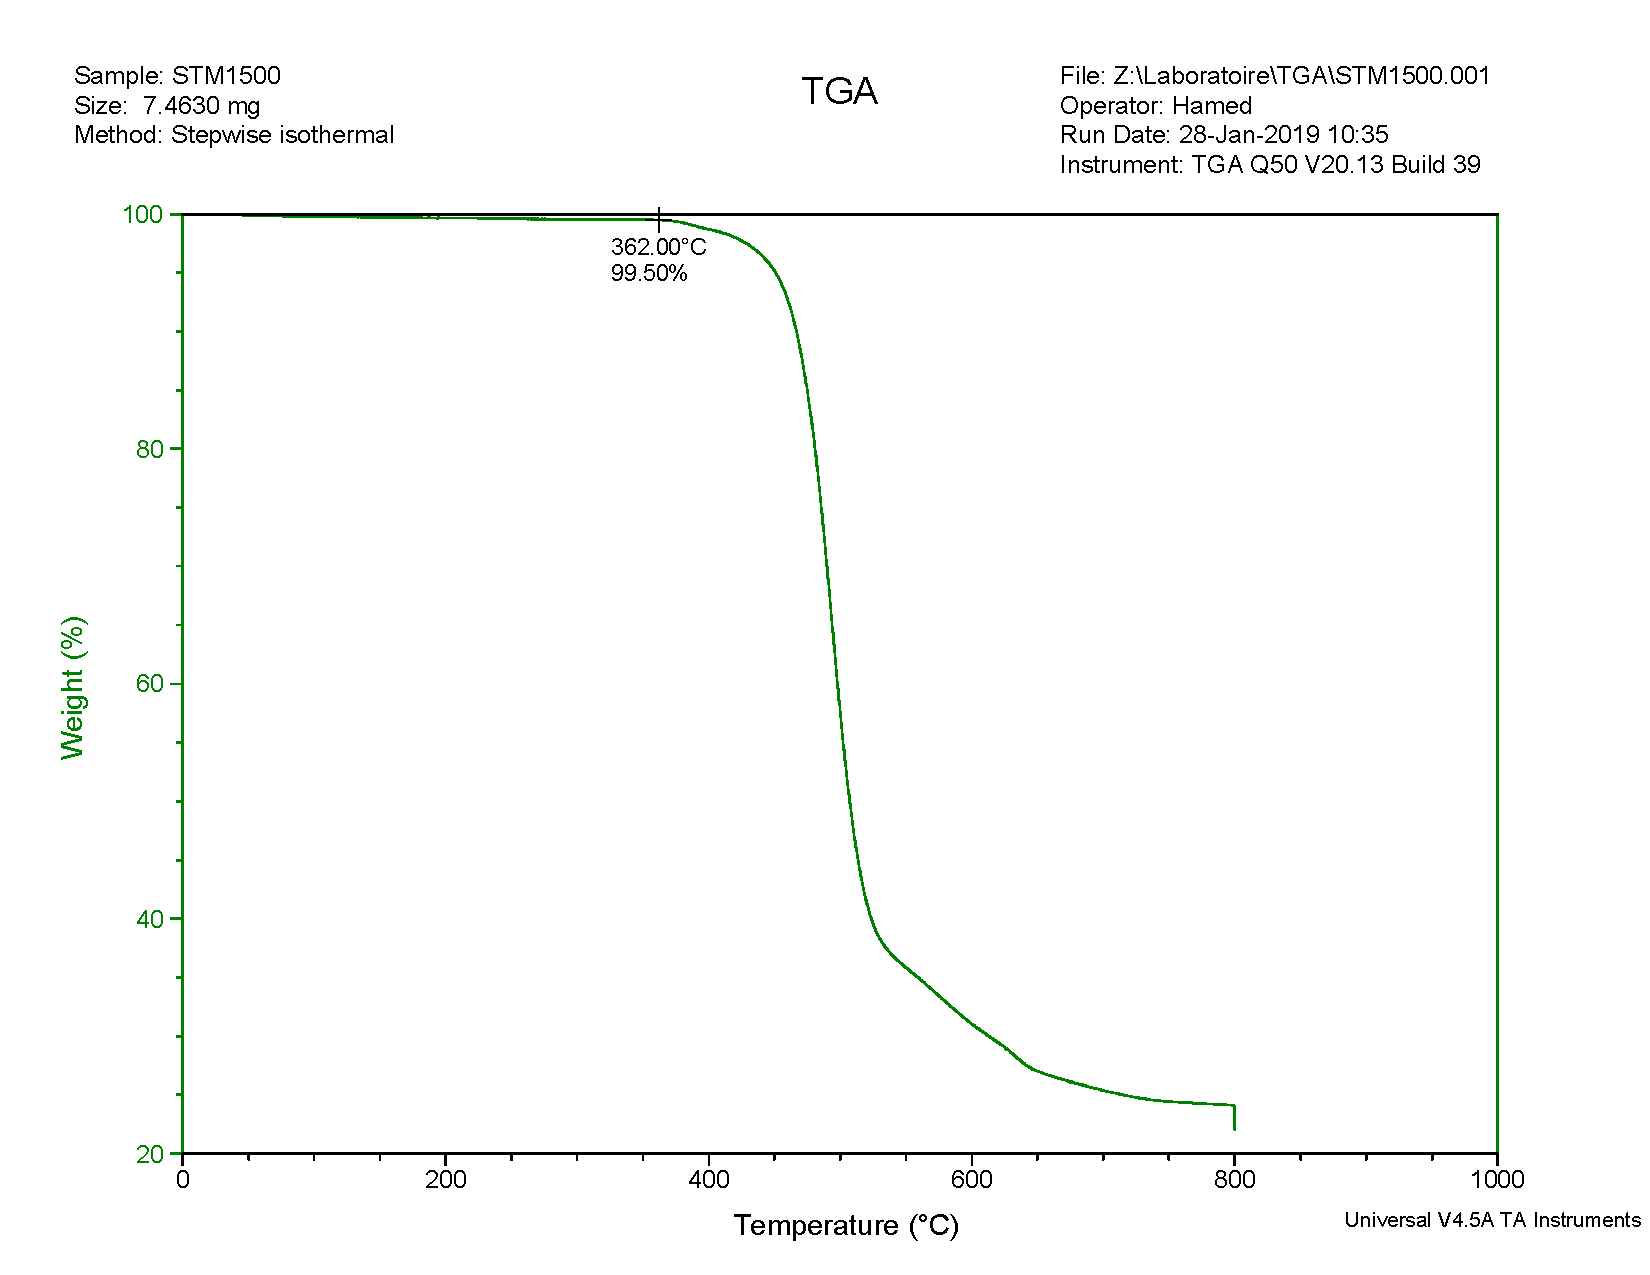
\includegraphics[width=0.95\textwidth]{TGA_STM1500.pdf}
	\caption{Résultats en TGA dans l'air pour le PEI-siloxane}
	\label{fig:TGA_STM1500}
\end{figure}

\FloatBarrier
\subsection{Caractérisation mécanique de l'élastomère}

Les échantillons de PEI-siloxane ont atteint une contrainte à la rupture de \SI[locale=FR]{29}{\mega\pascal} avec une déformation de 250\% (Fig. \ref{fig:STM1500_tension}). 

\begin{figure}[h]
	\centering
	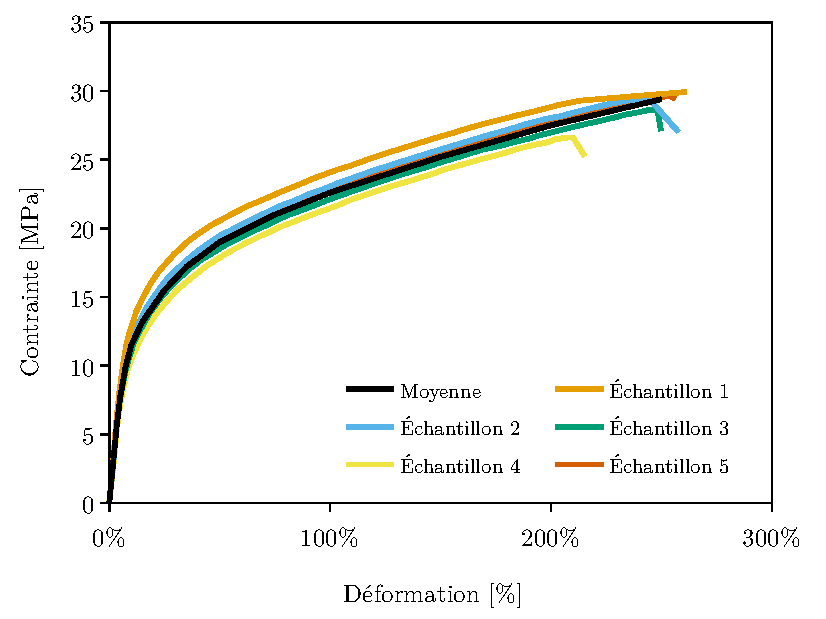
\includegraphics[width=0.7\textwidth]{STM1500_tension.pdf}
	\caption{Résultats des essais de traction pour le PEI-siloxane}
	\label{fig:STM1500_tension}
\end{figure}

\FloatBarrier
\subsection{Essais de soudage isotherme}

Les essais de soudage pour le PEI-siloxane ont débuté avec un essai dans une étuve sous vide. 
Un échantillon y a été inséré et chauffé jusqu'à \SI[locale=FR]{280}{\celsius} pendant 24 heures (Fig. \ref{fig:weldstack_STM1500}). 
À la sortie de l'étuve, l'échantillon était totalement plat (Fig. \ref{fig:etuve_STM1500_flat}), mais, après avoir séparé le nanocomposite du composite, une portion de l'élastomère ne pouvait être retirée (Fig.~\ref{fig:etuve_STM1500_adhesion}). 
En raison de la faible distance de diffusion des chaines de polymère, même lors d'un soudage réussi, il a été impossible de confirmer au microscope optique ou même par analyse atomique au microscope électronique à balayage la diffusion des chaines au travers de l'interface. 
Il est également possible de remarquer que, durant cet essai, la couleur de l'élastomère a changé, avec une transition de sa teinte vers le brun.  
Ce dernier signe démontre un début de dégradation thermique de l'élastomère lors d'une exposition prolongée à des températures élevées. 
Il est important de vérifier qu'un procédé plus court ne produira pas de dégradation de l'élastomère. 
La prochaine étape de cette validation pour le PEI-siloxane a été de produire une soudure dans une presse chauffante. 
À la fin de cet essai, encore une fois, en raison de la pression élevée, l'élastomère a presque totalement quitté la zone à souder (Fig. \ref{fig:welds_STM1500_presse}), mais, après séparation des composants, un film d'élastomère est resté fortement adhéré au nanocomposite (Fig. \ref{fig:welds_STm1500_presse_adhesion}). 
Cette fois par contre, le procédé, d'une durée approximative de \SI[locale=FR]{15}{\minute} en incluant le temps de refroidissement, a été assez rapide pour ne pas altérer la couleur de l'élastomère. 

\begin{figure}[h]
	\centering
	\subfigure[]
	{\label{fig:weldstack_STM1500} 								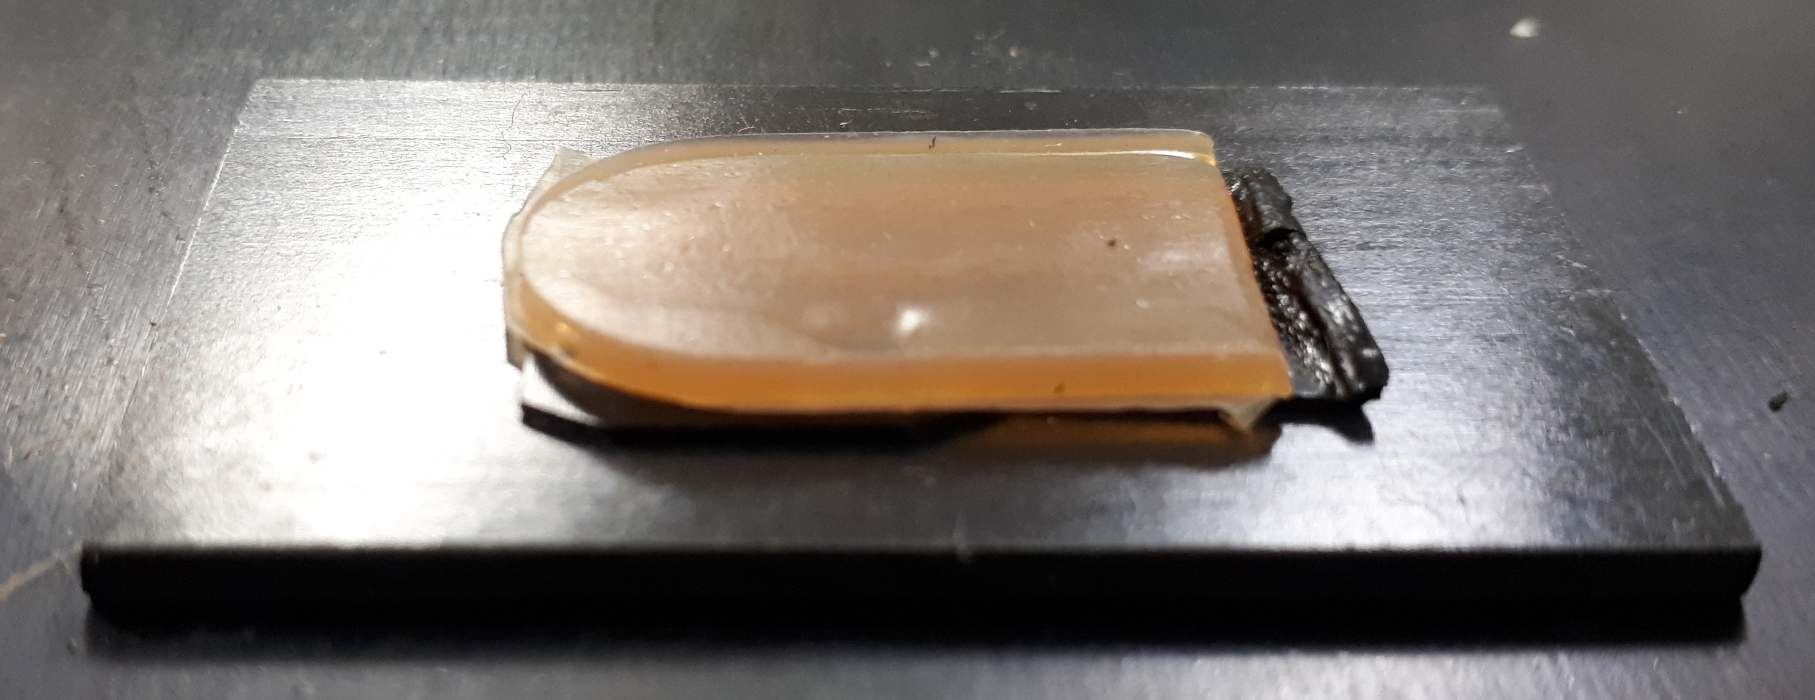
\includegraphics[height=3.6cm]{20181002_121017_crop_resize.jpg}	
	} \
	\subfigure[]
	{\label{fig:etuve_STM1500_flat} 								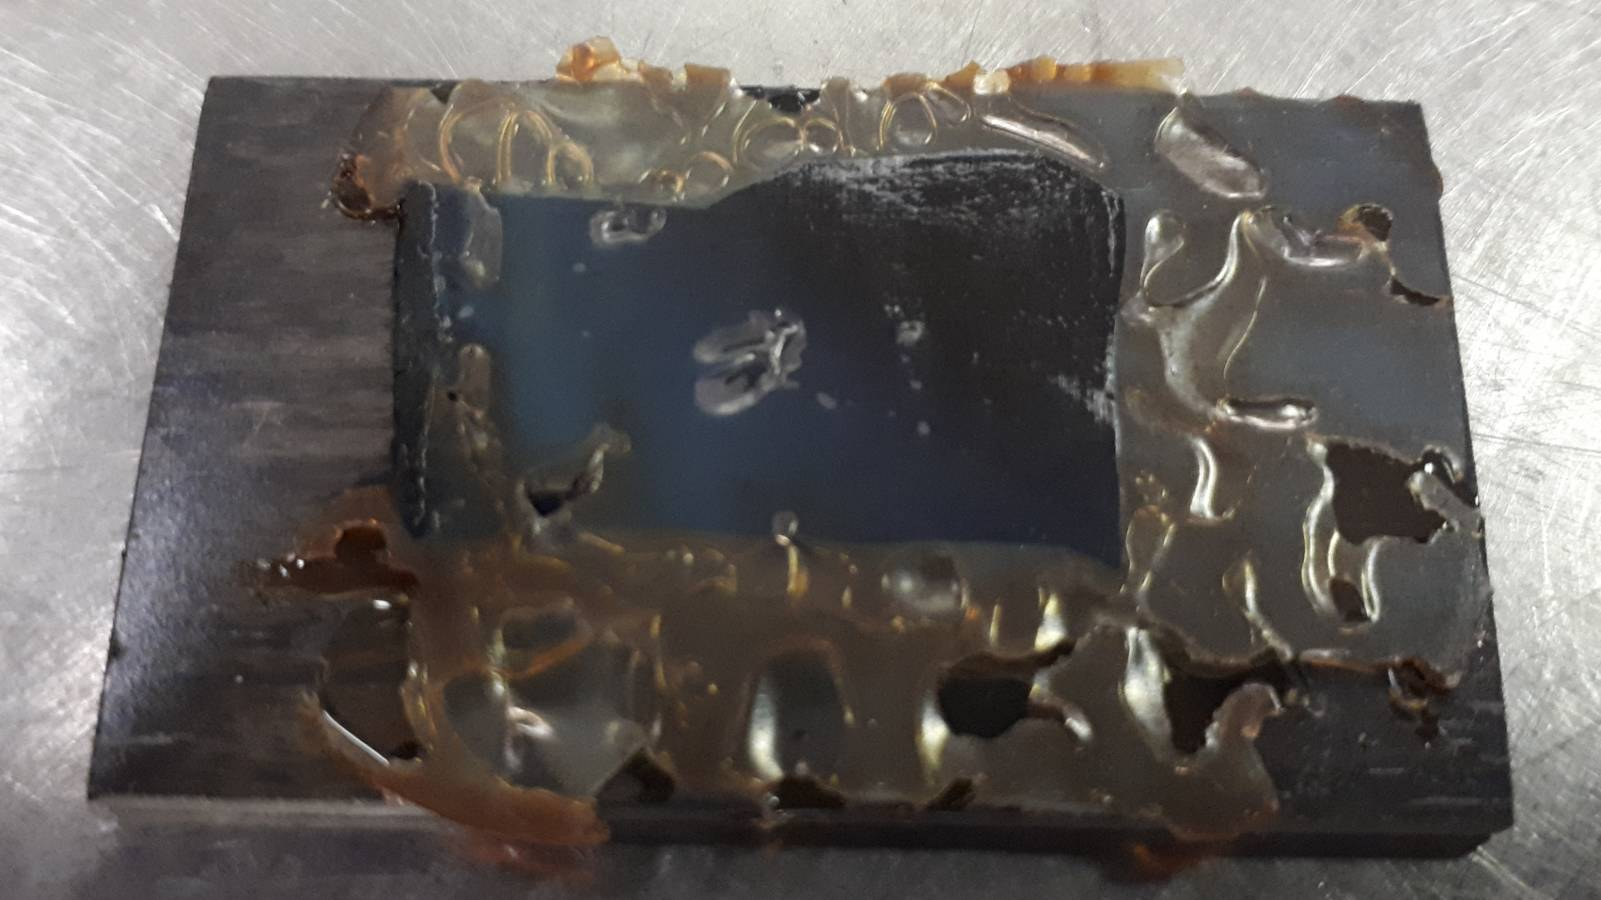
\includegraphics[height=3.6cm]{20181003_100733_crop_resize.jpg}
	} \
	\subfigure[]
	{\label{fig:etuve_STM1500_adhesion}
		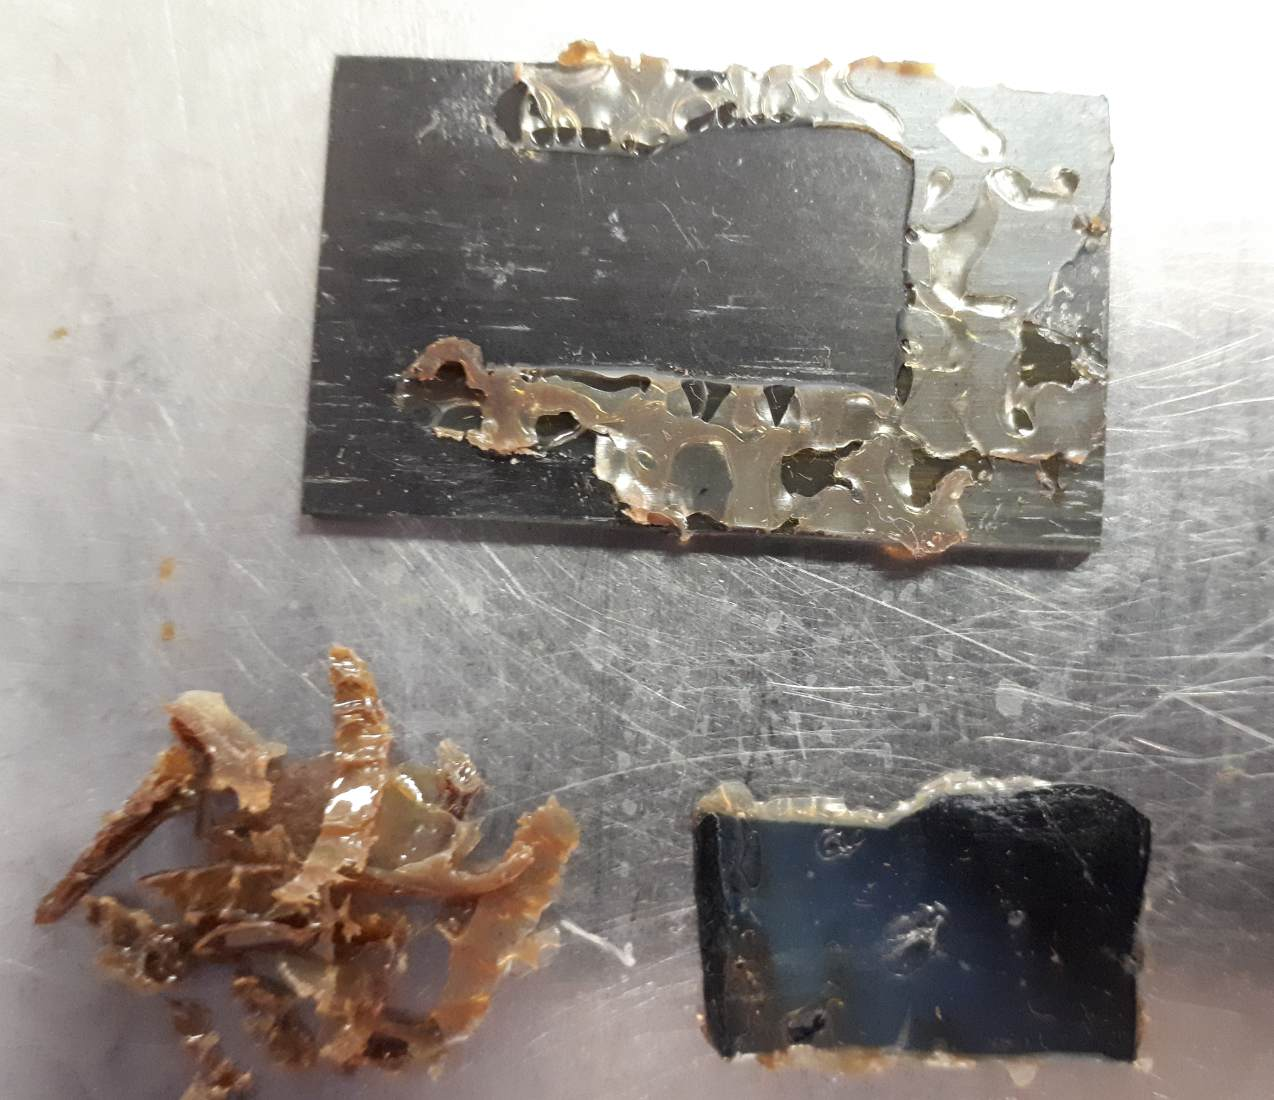
\includegraphics[height=3.6cm]{20181003_102113_crop_resize.jpg}
	}
	\caption{Essai de soudage dans une étuve sous vide à \SI{280}{\celsius} pour l'élastomère PEI-siloxane présentant a) la préparation de l'échantillon, b) l'échantillon à la sortie de l'étuve et c) l'adhésion de l'élastomère sur le nanocomposite}
	\label{fig:etuve_STM1500}
	
	\centering
	\subfigure[]
	{\label{fig:welds_STM1500_presse} 								
		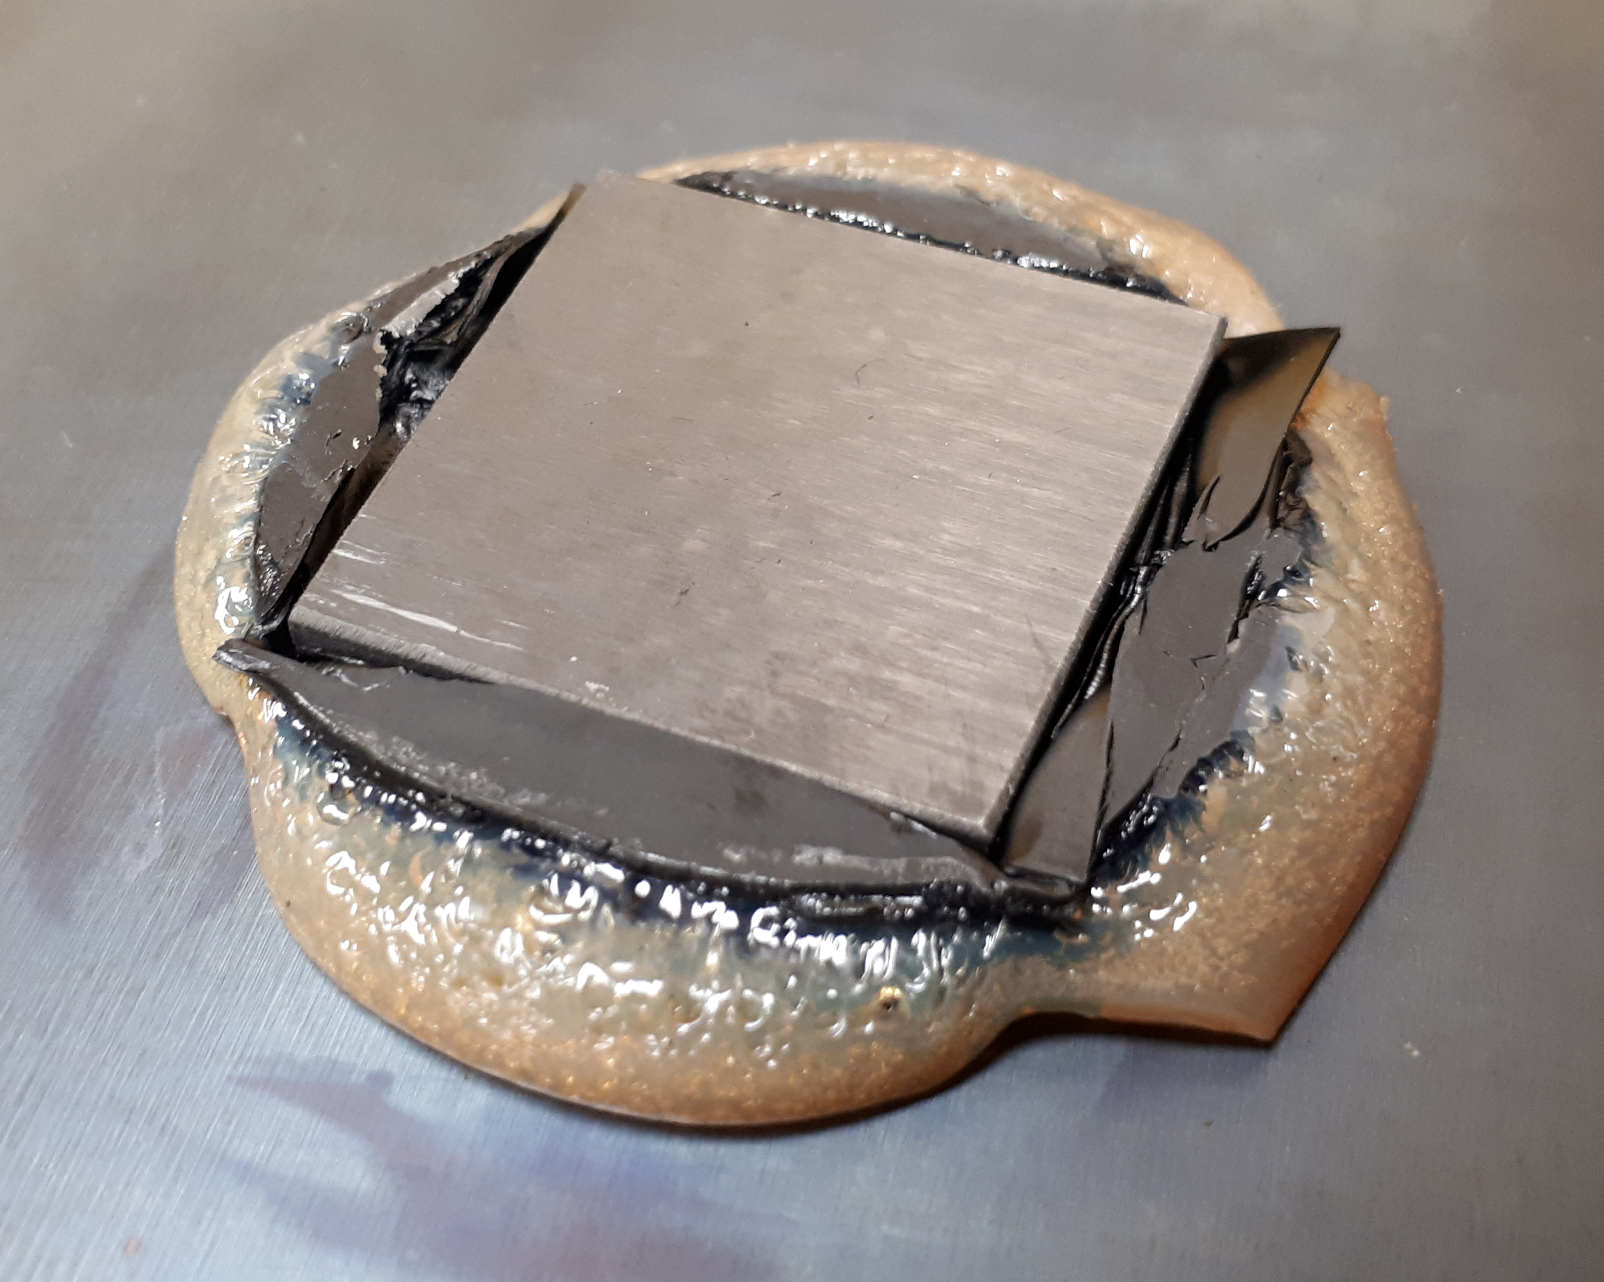
\includegraphics[height=4.5cm]{20181108_100951_crop_resize.jpg}
	} \qquad
	\subfigure[]
	{\label{fig:welds_STm1500_presse_adhesion} 								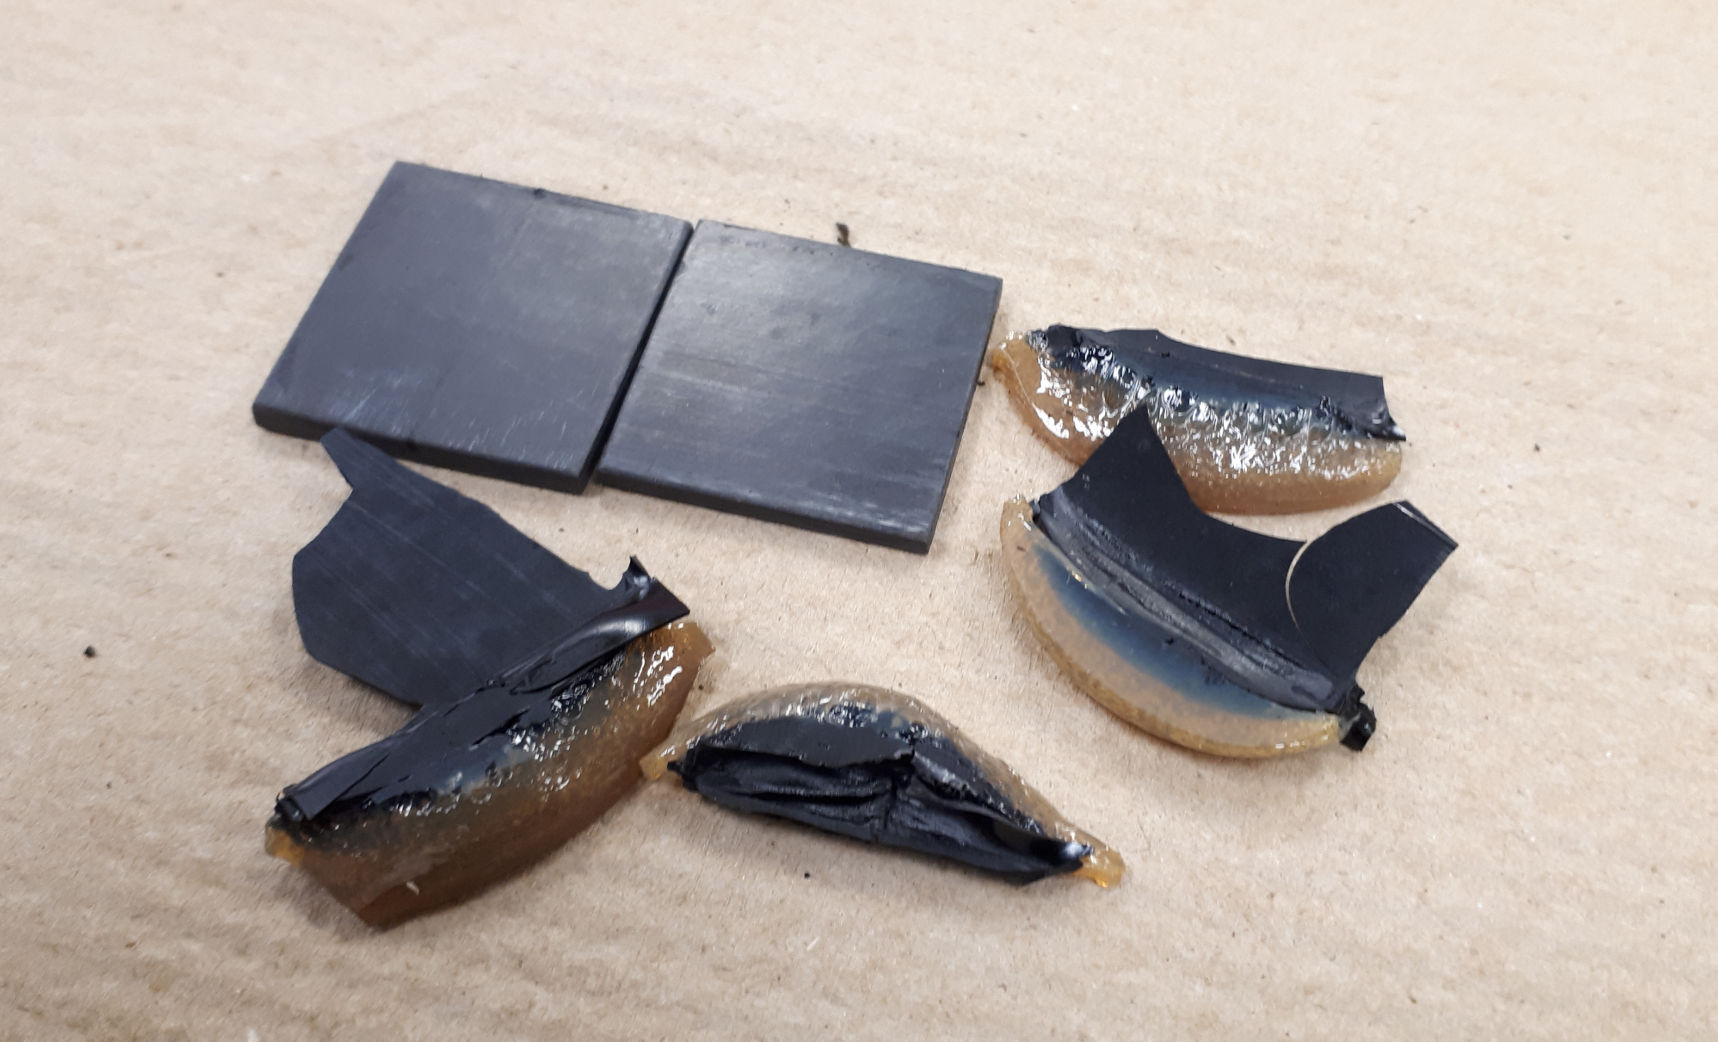
\includegraphics[height=4.5cm]{20181108_101250_resize_crop.jpg}
	}
	\caption{Essai de soudage à la presse à \SI{280}{\celsius} pour l'élastomère PEI-siloxane présentant a) l'échantillon à la sortie de la presse et b) l'adhésion de l'élastomère sur le nanocomposite}
	\label{fig:presse_STM1500}
\end{figure}

Un point intéressant à noter est que, malgré l'adhésion visible entre l'élastomère et le nanocomposite, le soudage entre le composite et le nanocomposite n'arrive pas à se produire aux températures employées lors des essais à l'étuve ou dans la presse. 
Ce comportement peut être lié à la quantité de charges dans le nanocomposite qui en viennent à affecter la mobilité des chaines de polymère. 
Ce même comportement avait été dénoté dans le chapitre \ref{sec:Theme2} et causait une augmentation de la température nécessaire pour le soudage. 
Cet indice porte à croire que les températures d'opération pour les deux types de soudage ne seront pas nécessairement compatibles. 

\FloatBarrier

\subsection{Évaluation de la vitesse de dégradation thermique du PEI-siloxane}

Afin de déterminer un temps maximal pour le soudage, il est nécessaire d'évaluer plus précisément la vitesse de dégradation thermique du PEI-siloxane. 
Un mélange composé de PEI et de 10\% d'élastomère a été produit. 
Lors de ce test, le PEI a été mélangé avec une vitesse de rotation de 150 RPM jusqu'à ce que la température du mélange se stabilise à \SI[locale=FR]{350}{\celsius}. 
Les granules de PEI-siloxane ont alors été ajoutées et le couple du rotor a été enregistré en continu pendant 40 minutes (Fig. \ref{fig:STM1500_thermo_Haake_couple}). 
On peut voir qu'après une fonte rapide, le couple remonte progressivement pour atteindre un plateau avec une légère pente aux alentours de \SI[locale=FR]{600}{\second} (10 minutes). 
Ce plateau se poursuit pendant 15 minutes, soit jusqu'à approximativement \SI[locale=FR]{1500}{\second} (25 minutes), avant que la viscosité ne commence à augmenter de plus en plus rapidement. 
L'élastomère recueilli après cet essai présentait des signes flagrants de dégradation thermique (Fig. \ref{fig:STM1500_thermo_Haake_degradation}). 
Ces résultats permettent de confirmer que la stabilité thermique du PEI-siloxane est suffisante pour réaliser des soudures à condition que la température soit gardée sous contrôle. 

\begin{figure}[h]	
	\centering
	\subfigure[]
	{\label{fig:STM1500_thermo_Haake_couple} 								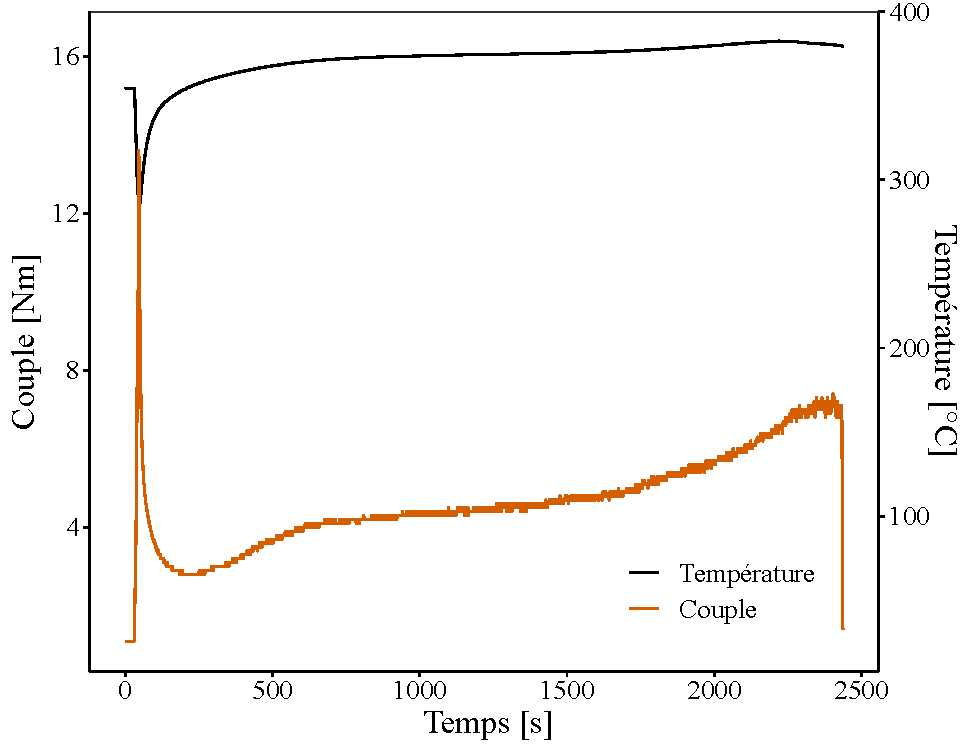
\includegraphics[height=7cm]{thermo_haake_STM1500.pdf}
	} \qquad
	\subfigure[]
	{\label{fig:STM1500_thermo_Haake_degradation}
		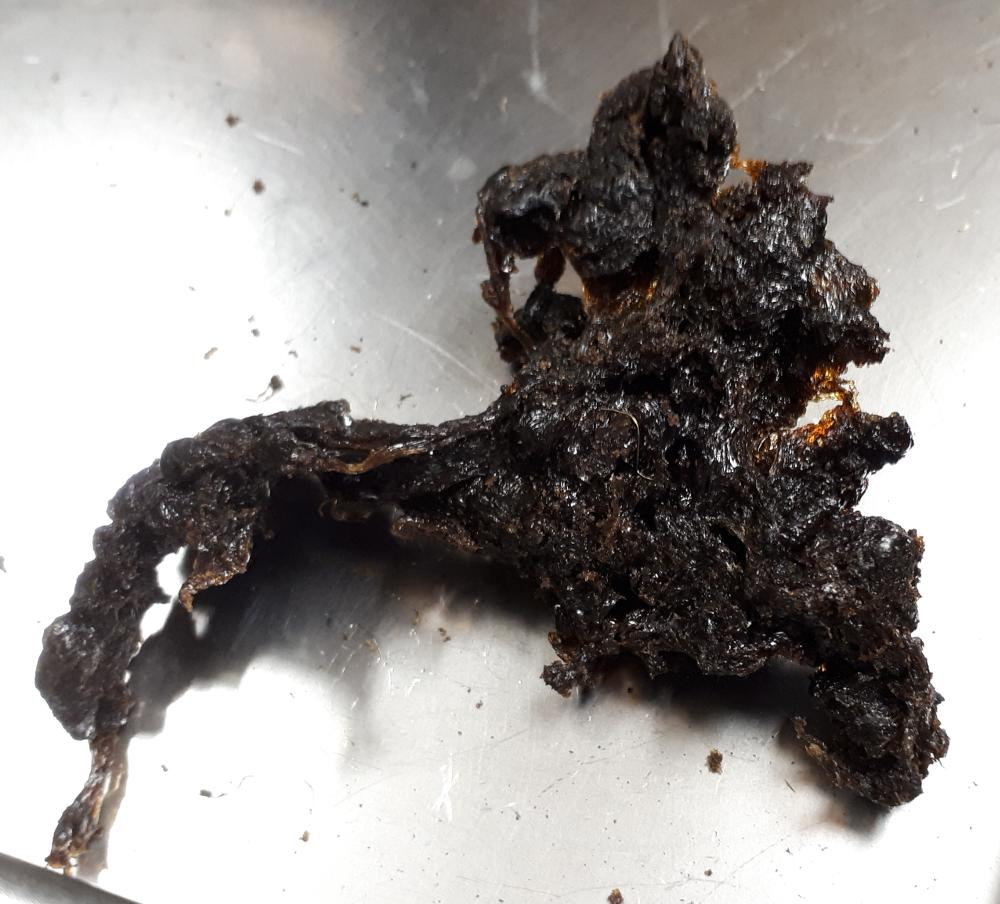
\includegraphics[height=5.cm]{20190822_110329_crop_resize.jpg}
	} \\
	\caption{Évaluation de la stabilité thermique du PEI-siloxane à l'aide d'un mélangeur interne présentant a) l'évolution du couple pendant le mélange et b) l'état de dégradation de l'élastomère après 40 minutes}
	\label{fig:STM1500_thermo_Haake}
\end{figure}

Une analyse des mécanismes de dégradation serait nécessaire pour expliquer les raisons menant à la variation de couple lors de cet essai. 
Il n'a pas été possible de trouver de telles analyses dans la littérature pour le PEI-siloxane. 
Par contre, en ce qui concerne le siloxane, au-dessus de \SI{180}{\celsius}, la dégradation de ce polymère produit un raccourcissement des chaines par la scission de liaisons Si--O  et la formation de groupes cycliques de siloxane avec une faible l'élasticité \cite{Heinemann2004}. 
Une exposition prolongée à de hautes températures cause une dégradation du réseau siloxane et une augmentation de la rigidité du polymère. 
Ce mécanisme pourrait expliquer le comportement observé.  

\FloatBarrier

\subsection{Essais de soudage par résistance}

Un premier essai a été réalisé dans le montage de soudage par résistance à l'aide de petits échantillons d'élastomère et de composite ainsi que d'un élément chauffant nanocomposite. 
L'échantillon a été installé dans le montage de soudage (Fig. \ref{fig:STM1500_soudure_montage}) et un essai de soudage a été réalisé avec une puissance surfacique de \SI[locale=FR]{260}{\kilo\watt\per\square\metre} pendant \SI[locale=FR]{60}{\second}. 
Une jonction a été obtenue en une seule étape lors de cet essai. 
Les tentatives pour séparer l'élastomère ont, encore une fois, permis de séparer le nanocomposite du composite, mais sans permettre de séparer l'élastomère du nanocomposite. 
En raison de l'absence de soudure entre les adhérents composites et les éléments chauffants nanocomposites, la méthode de soudure en une étape a été abandonnée.
Les essais subséquents ont utilisé un mode de soudure en deux étapes où l'élément chauffant était préalablement soudé sur un adhérent composite. 

\FloatBarrier
\begin{figure}[h]
	\centering
	\subfigure[]
	{\label{fig:STM1500_soudure_montage} 								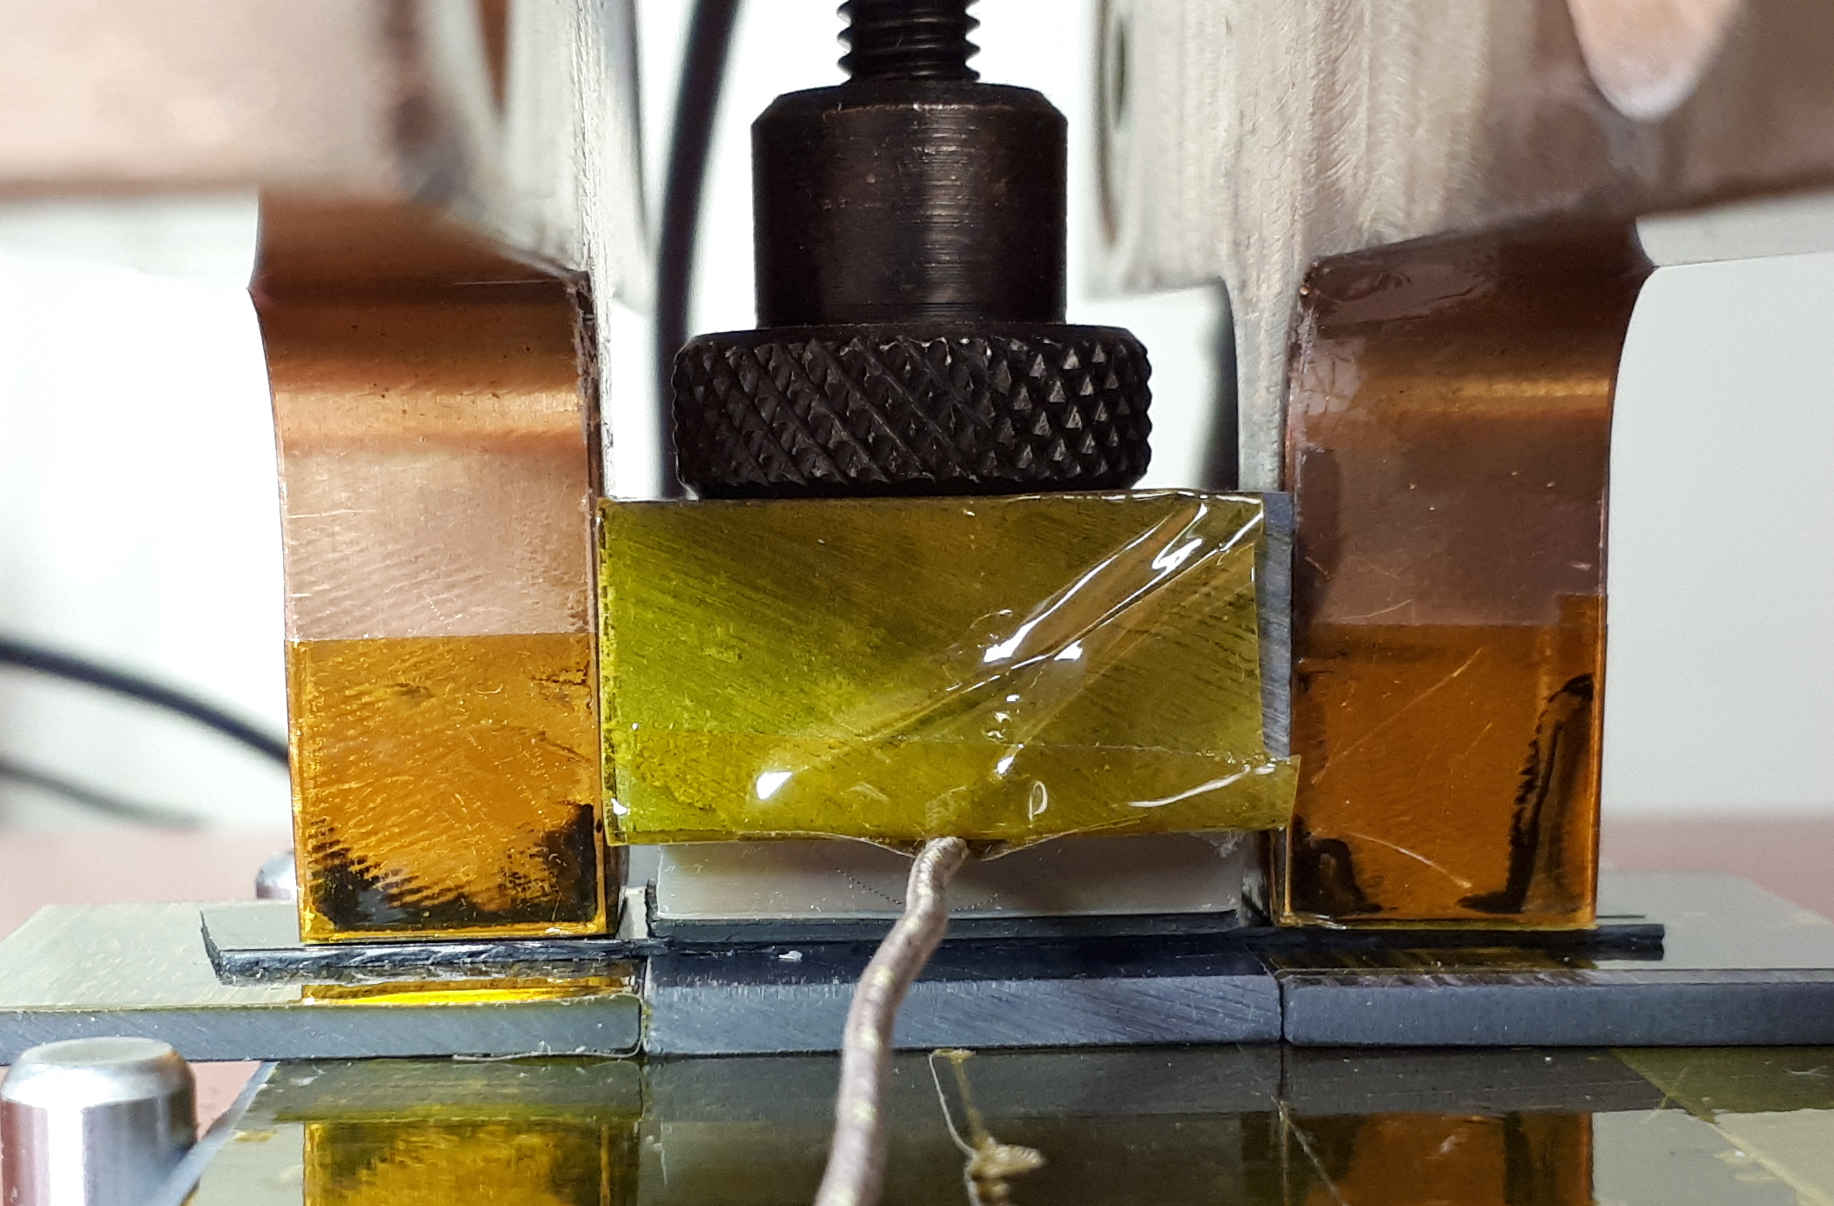
\includegraphics[height=4.25cm]{20181109_111133_crop_resize.jpg}
	} \qquad
	\subfigure[]
	{\label{fig:STM1500_soudure_resultat}
		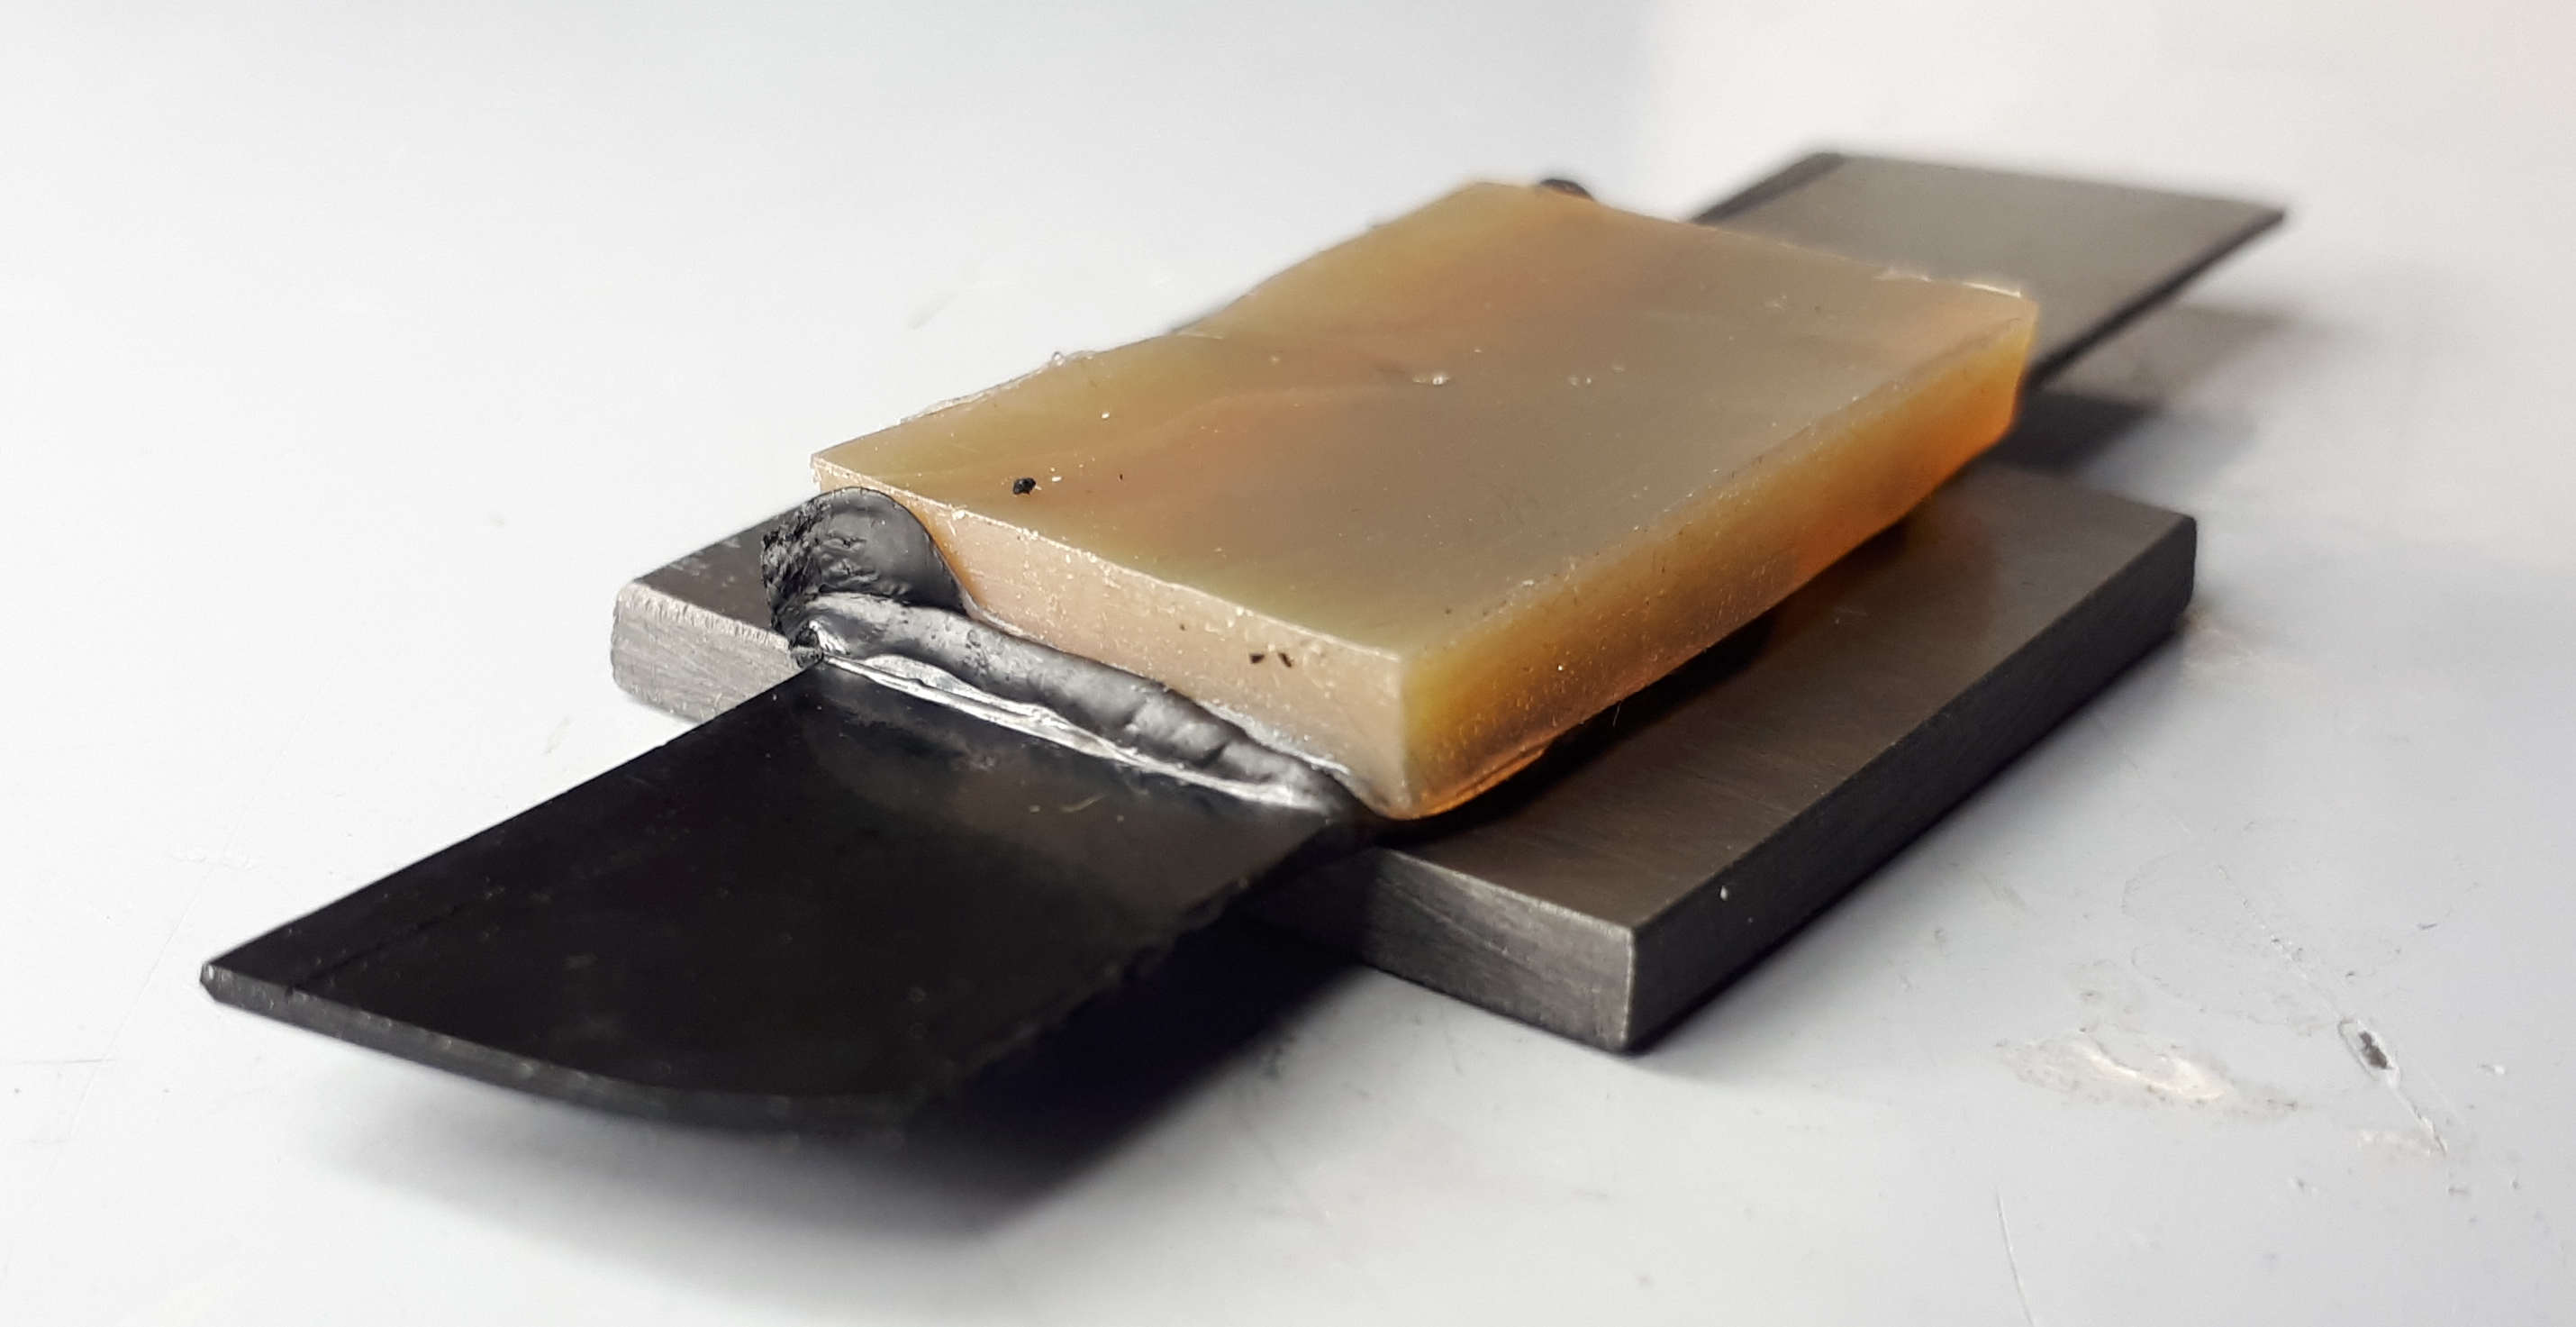
\includegraphics[height=4.25cm]{20181109_113850_crop.jpg}
	}
	\caption{Essai de soudage d'un échantillon avec l'élastomère PEI-siloxane avec a) l'échantillon positionné dans le montage de soudage et b) le résultat de l'essai de soudage}
	\label{fig:STM1500_soudure}
\end{figure}
\FloatBarrier

Une série de soudures exploratoires ont été réalisées afin de cerner une fenêtre d'opération. 
Lors des essais initiaux, des thermocouples étaient installés pour mesurer l'élévation de température sur la face opposée de l'élastomère. 
Les essais étaient arrêtés si la température s'élevait rapidement au-dessus des températures pouvant causer une dégradation rapide de l'élastomère ou un fluage prononcé de l'élastomère en dehors de la zone soudée. 
Les deux premiers essais à 260 et \SI[locale=FR]{220}{\kilo\watt\per\square\metre} ont dû être arrêtés après seulement \SI[locale=FR]{60}{\second} en raison de dégagements de fumée (Fig. \ref{fig:MM_260_60} et \ref{fig:MM_220_60}). 
Dans les deux cas, l'élastomère a pu être facilement arraché de la jonction après la soudure et on pouvait voir des signes de dégradation de l'élastomère et du nanocomposite. 
Il était alors nécessaire de considérer deux options: souder à plus faible puissance pendant un temps prolongé ou souder brièvement à haute puissance. 
Le troisième essai a été réalisé à une plus faible puissance de \SI[locale=FR]{180}{\kilo\watt\per\square\metre} pendant \SI[locale=FR]{180}{\second} (Fig. \ref{fig:MM_180_180}). 
L'essai a été arrêté lorsque la face supérieure a atteint la température de \SI[locale=FR]{120}{\celsius}. 
Pour cet échantillon, il a été possible de séparer aisément l'élastomère du nanocomposite et aucun signe de diffusion n'a été noté. 
Finalement pour l'approche avec un temps court et une puissance élevée, un échantillon a été produit avec une puissance surfacique de \SI[locale=FR]{300}{\kilo\watt\per\square\metre} et un temps de \SI[locale=FR]{45}{\second}. 
La rupture de l'élastomère pour cet essai s'est produite dans l'adhérent et une portion de l'élastomère est resté adhéré. 
Cette dernière condition de test a été répétée avec des adhérents sur des substrats métalliques. 
Les essais subséquents ont également utilisé des conditions similaires. 

\FloatBarrier
\begin{figure}[h]
	\centering
	\subfigure[]
	{\label{fig:MM_260_60} 								
		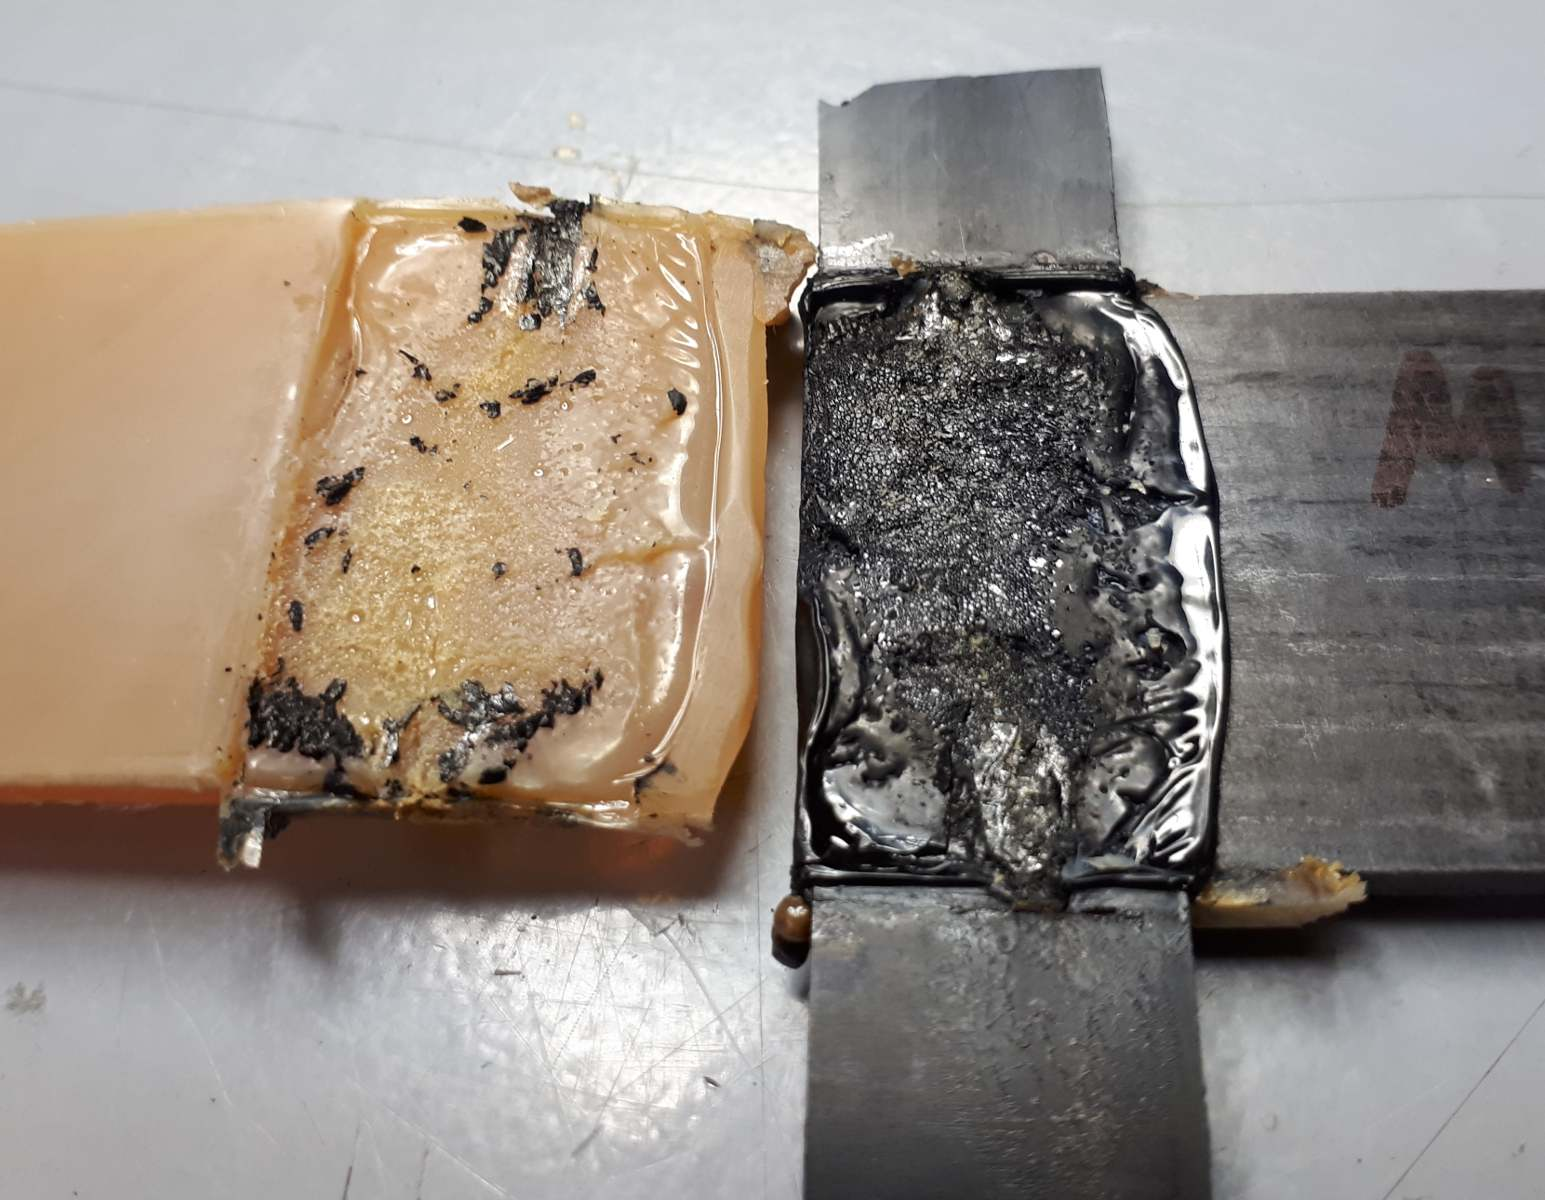
\includegraphics[height=5.5cm]{MM_260_60_crop_resize.jpg}
	} \qquad
	\subfigure[]
	{\label{fig:MM_220_60}
		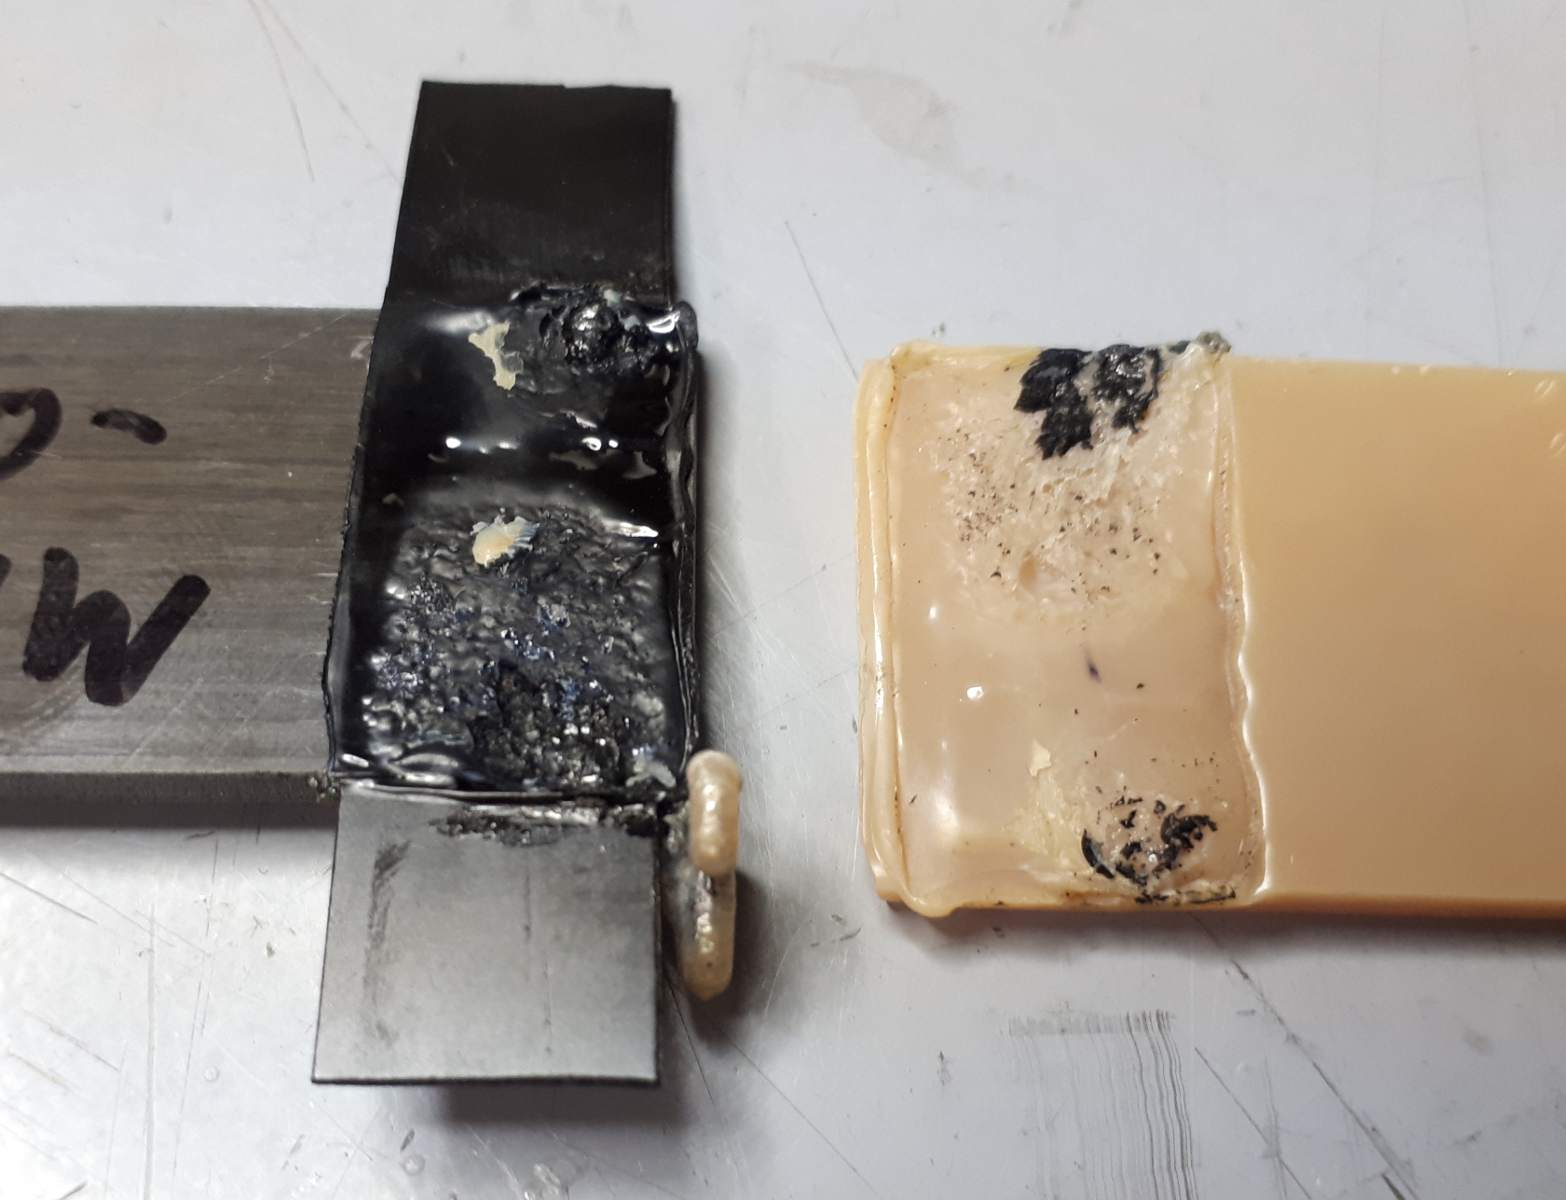
\includegraphics[height=5.5cm]{MM_220_60_crop_resize.jpg}
	} \\
	
	\subfigure[]
	{\label{fig:MM_180_180} 		
		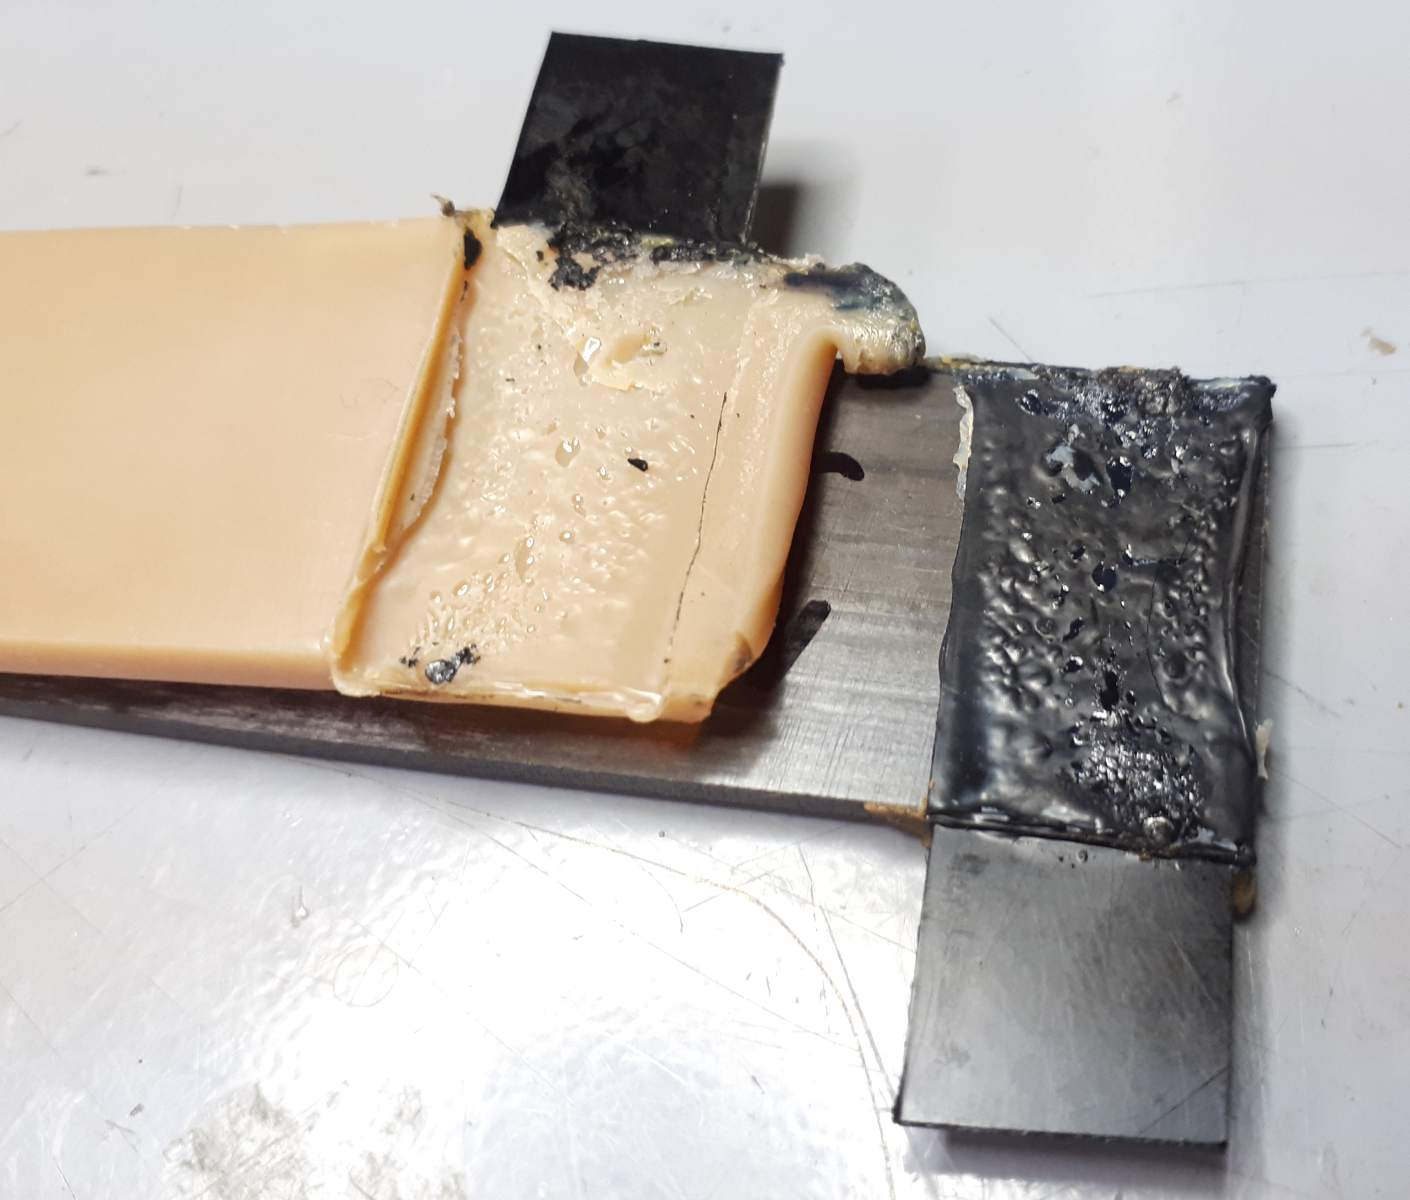
\includegraphics[height=5.5cm]{MM_180_180_crop_resize.jpg}
	} \qquad
	\subfigure[]
	{\label{fig:MM_300_45}
		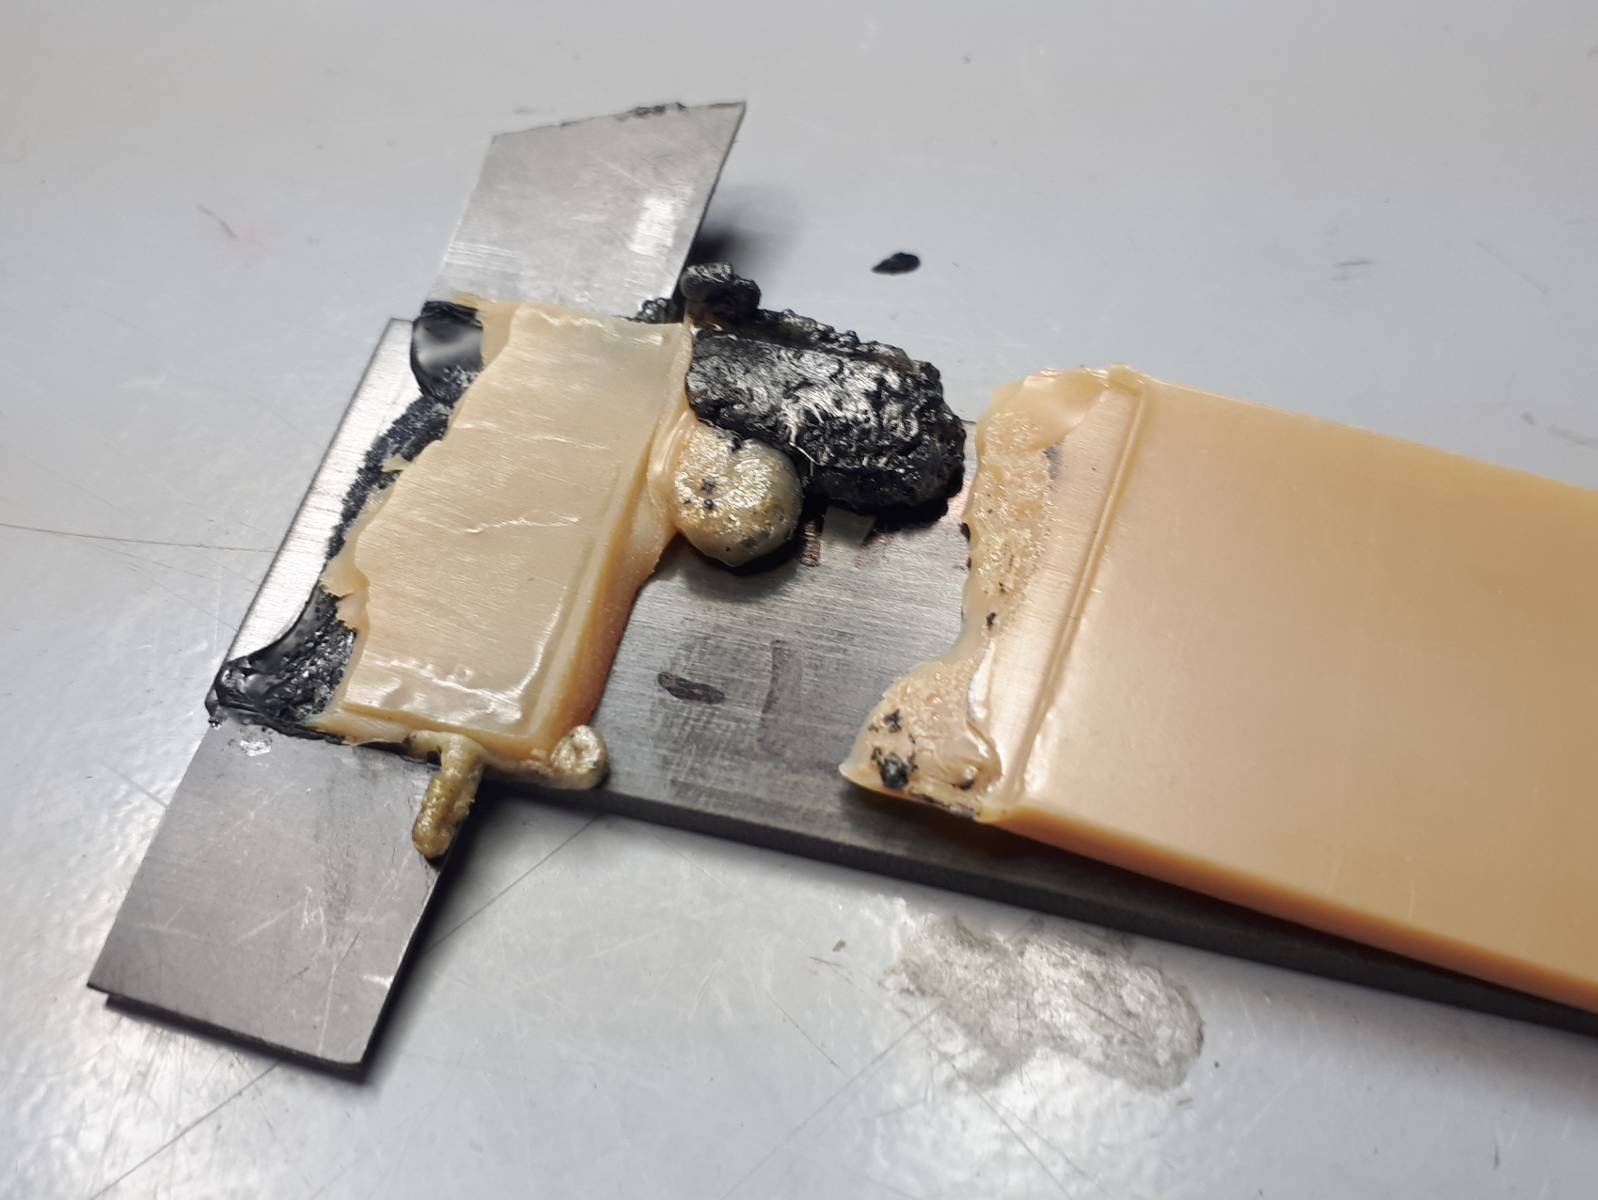
\includegraphics[height=5.5cm]{MM_300_45_crop_resize.jpg}
	} 
	\caption{Résultats des essais de soudage multimatériaux initiaux avec des paramètres de soudage à a) \SI{260}{\kilo\watt\per\square\metre} pendant \SI{60}{\second}, b) \SI{220}{\kilo\watt\per\square\metre} pendant \SI{60}{\second}, c) \SI{180}{\kilo\watt\per\square\metre} pendant \SI{180}{\second} et d) \SI{300}{\kilo\watt\per\square\metre} pendant \SI{45}{\second}}
	\label{fig:MM_essais_initiaux}
\end{figure}
\FloatBarrier

La résistance des soudures obtenues a pu être évaluée par essais de simple cisaillement (Tab.~\ref{tab:LSS_multi_materiau}). 
Des temps de soudage de 35 et \SI[locale=FR]{45}{\second} ainsi que des puissances entre 220 et \SI[locale=FR]{300}{\kilo\watt\per\square\metre} ont été utilisés et permettaient d'obtenir des soudures. 
La pression sur la soudure a été réduite après les deux premières conditions de test en raison de la quantité de polymère ayant flué. 
Dans tous les cas, sauf pour la soudure réalisée avec une puissance de \SI[locale=FR]{220}{\kilo\watt\per\square\metre}, une fumée blanche a été dégagée durant le soudage. 

\begin{table}[h]
	\centering
	\caption{Essais de caractérisation mécanique de soudures multimatériaux}
	\begin{tabular}{@{}cccC{1in}c@{}}
		\toprule
		Puissance                &       Temps        &        Pression         & Nombre d'échantillons &    LSS (Écart-type)     \\
		{[}\si{\kilo\watt\per\square\metre}{]} & {[}\si{\second}{]} & {[}\si{\mega\pascal}{]} &                       & {[}\si{\mega\pascal}{]} \\ \midrule
		300                   &         45         &            1            &           1           &       8,2 (S.O.)        \\
		300                   &         35         &            1            &           1           &       5,7 (S.O.)        \\
		300                   &         45         &           0,4           &           5           &        6,3 (1,0)        \\
		280                   &         45         &           0,4           &           2           &        4,2 (0,1)        \\
		260                   &         45         &           0,4           &           2           &        4,6 (0,8)        \\
		240                   &         45         &           0,4           &           2           &        2,6 (0,7)        \\
		220                   &         45         &           0,4           &           2           &        2,0 (0,2)        \\ \bottomrule
	\end{tabular}
	\label{tab:LSS_multi_materiau}
\end{table}

\begin{figure}[h]
	\centering
	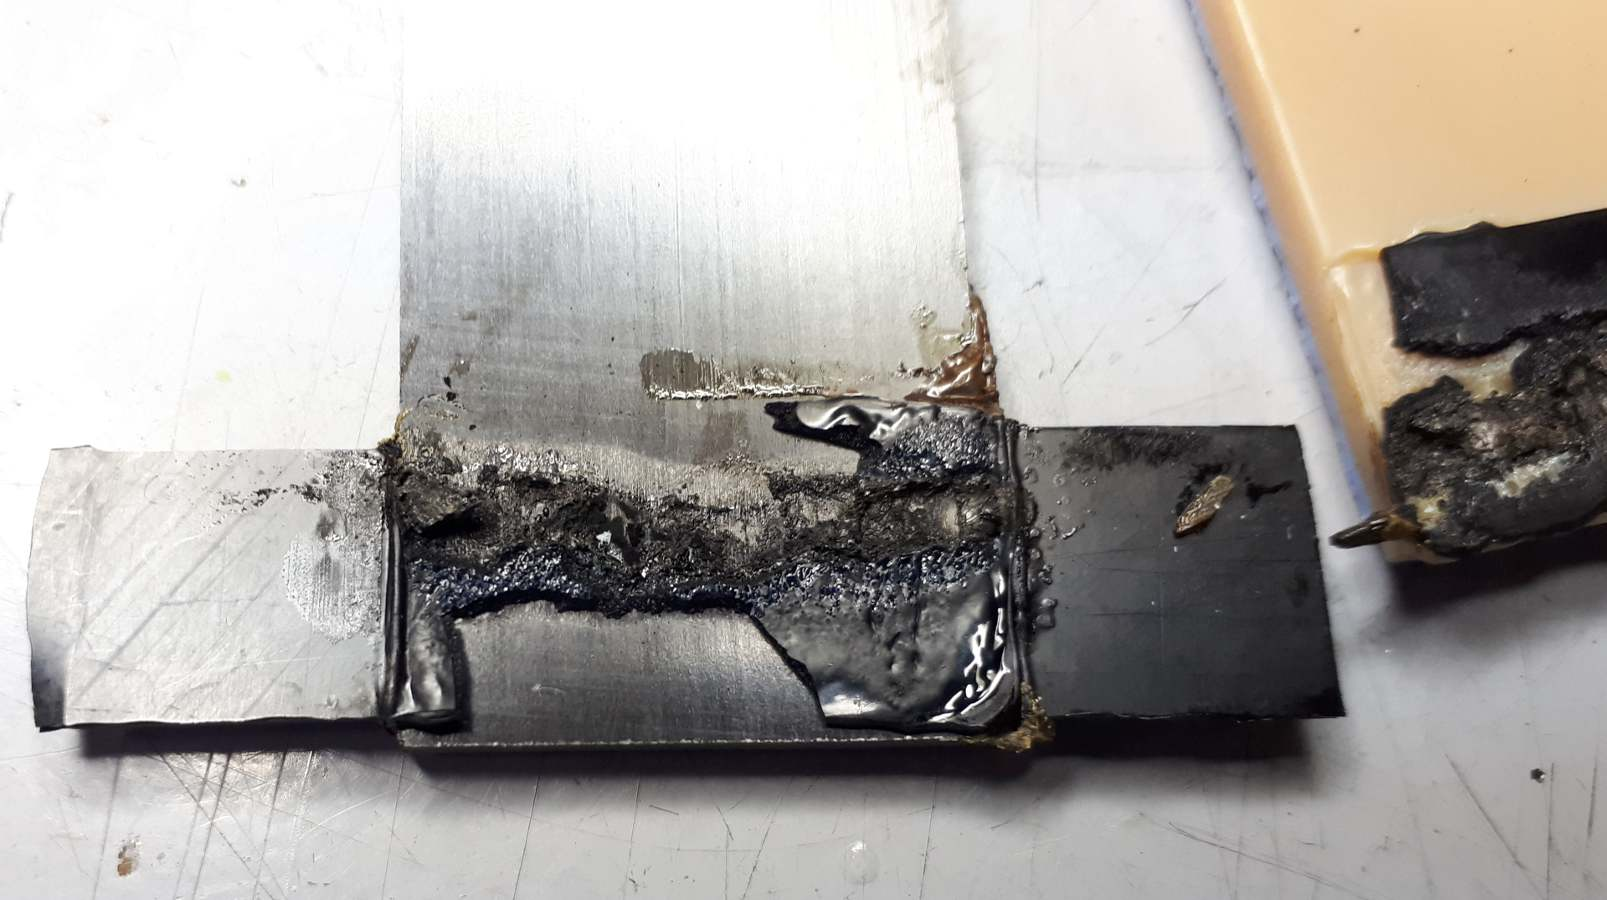
\includegraphics[width=0.5\textwidth]{20190618_145038_crop_resize.jpg}
	\caption{Faciès de rupture après un essai mécanique d'une soudure multimatériaux}
	\label{fig:facies_multi_materiau}
\end{figure}

Une analyse des faciès de rupture des échantillons (Fig. \ref{fig:facies_multi_materiau}) permet de voir que des conditions de soudage sous-optimales entraînent la dégradation thermique du nanocomposite. 
Sur cette figure, on peut observer une section centrale fortement dégradée ainsi que des résidus adhérés à l'élastomère. 
Une observation au microscope optique a également révélé la formation de bulles et de porosités dans l'élastomère. 

La seconde série de tests employant des puissances réduites avait pour but de déterminer une puissance propice à générer une soudure, mais qui ne mènerait pas à une dégradation thermique de l'élastomère. 
L'observation des faciès obtenus lors de cette série de tests a permis de récolter un grand nombre d'informations. 
La demi-soudure entre l'élément chauffant nanocomposite et le composite a généralement été le point faible des soudures. 
Celle-ci doit en effet atteindre un état pleinement soudé après la réalisation des deux joints, mais sans atteindre la dégradation thermique. 
Il est nécessaire d'optimiser les paramètres de la première soudure en fonction de la puissance qui est appliquée lors de la deuxième soudure. 
Pour les joints produits avec des puissances de 260 et \SI[locale=FR]{280}{\kilo\watt\per\square\metre}, la rupture s'est produite dans le nanocomposite, du côté du composite. 
Pour ces puissances, la seconde étape de soudage a permis de compléter partiellement la première soudure. 
Pour les essais avec des puissances de 220 et \SI[locale=FR]{240}{\kilo\watt\per\square\metre}, la seconde étape de soudure n'a pas permis de compléter le premier joint.
Les ruptures se sont alors produites entre le nanocomposite et le composite. 
Du côté de l'élastomère, à partir de \SI[locale=FR]{220}{\kilo\watt\per\square\metre}, il y a formation d'un nombre croissant de porosités en fonction de la puissance appliquée. 
À partir de \SI[locale=FR]{240}{\kilo\watt\per\square\metre}, des résidus d'élastomères ont été laissés sur le nanocomposite. 
Ces résidus semblent se former lorsque la quantité de porosité à proximité de la surface de l'élastomère permet la formation d'une pellicule selon le mécanisme présenté à la figure \ref{fig:bulles_elastomere}. 
La présence de ces résidus adhérés au nanocomposite semble indiquer la possibilité d'obtenir une soudure entre les matériaux. 

\begin{figure}[h]
	\centering
	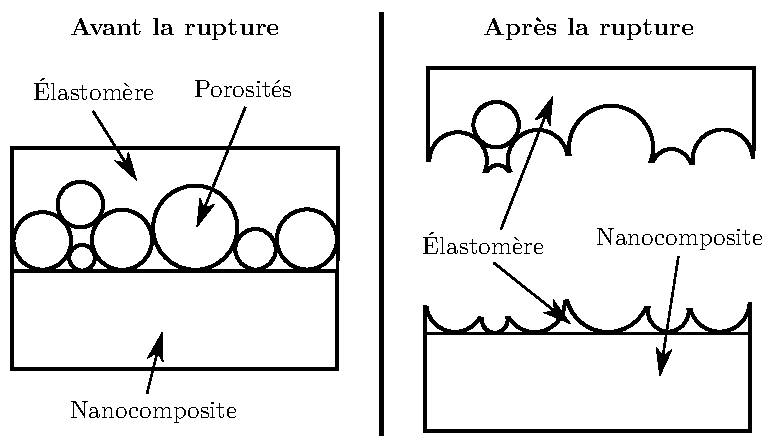
\includegraphics[scale=1]{bulles_elastomee.pdf}
	\caption{Mécanisme de rupture de l'élastomère après une soudure multimatériaux}
	\label{fig:bulles_elastomere}
\end{figure}

Afin d'éliminer tout problème pouvant avoir pour cause le nanocomposite, une soudure avec un élément chauffant en acier inoxydable a été produite. 
Pour cette soudure, une couche de PEI vierge a été laminée en surface des adhérents composites.
Un élément chauffant en grillage d'acier inoxydable a été inséré entre les adhérents de composite et d'élastomère. 
Un essai initial a été réalisé avec un thermocouple pour valider la température à l'interface. 
Avec une puissance de \SI[locale=FR]{220}{\kilo\watt\per\square\metre}, la température atteint \SI[locale=FR]{320}{\celsius} après \SI[locale=FR]{45}{\second} et \SI[locale=FR]{360}{\celsius} après \SI[locale=FR]{65}{\second}. 
Les résistances mécaniques de deux échantillons, soudés avec des puissances de 200 et \SI[locale=FR]{220}{\kilo\watt\per\square\metre} pendant \SI[locale=FR]{45}{\second}, ont été évaluées respectivement à 5,6 et \SI[locale=FR]{6,9}{\mega\pascal}. 
Une observation au microscope a permis d'observer un grand nombre de porosités dans le faciès de rupture. 
Encore une fois, les porosités à l'interface, cette fois combinées à la présence du grillage d'acier inoxydable, ont causé une rupture cohésive de l'élastomère au niveau de l'élément chauffant. 
Outre la présence de porosités, le résidu d'élastomère semble bien adhérer au composite.  

\begin{figure}[h]
	\centering
	\subfigure[]
	{\label{fig:STM1500_facies1_soudure_SS}
		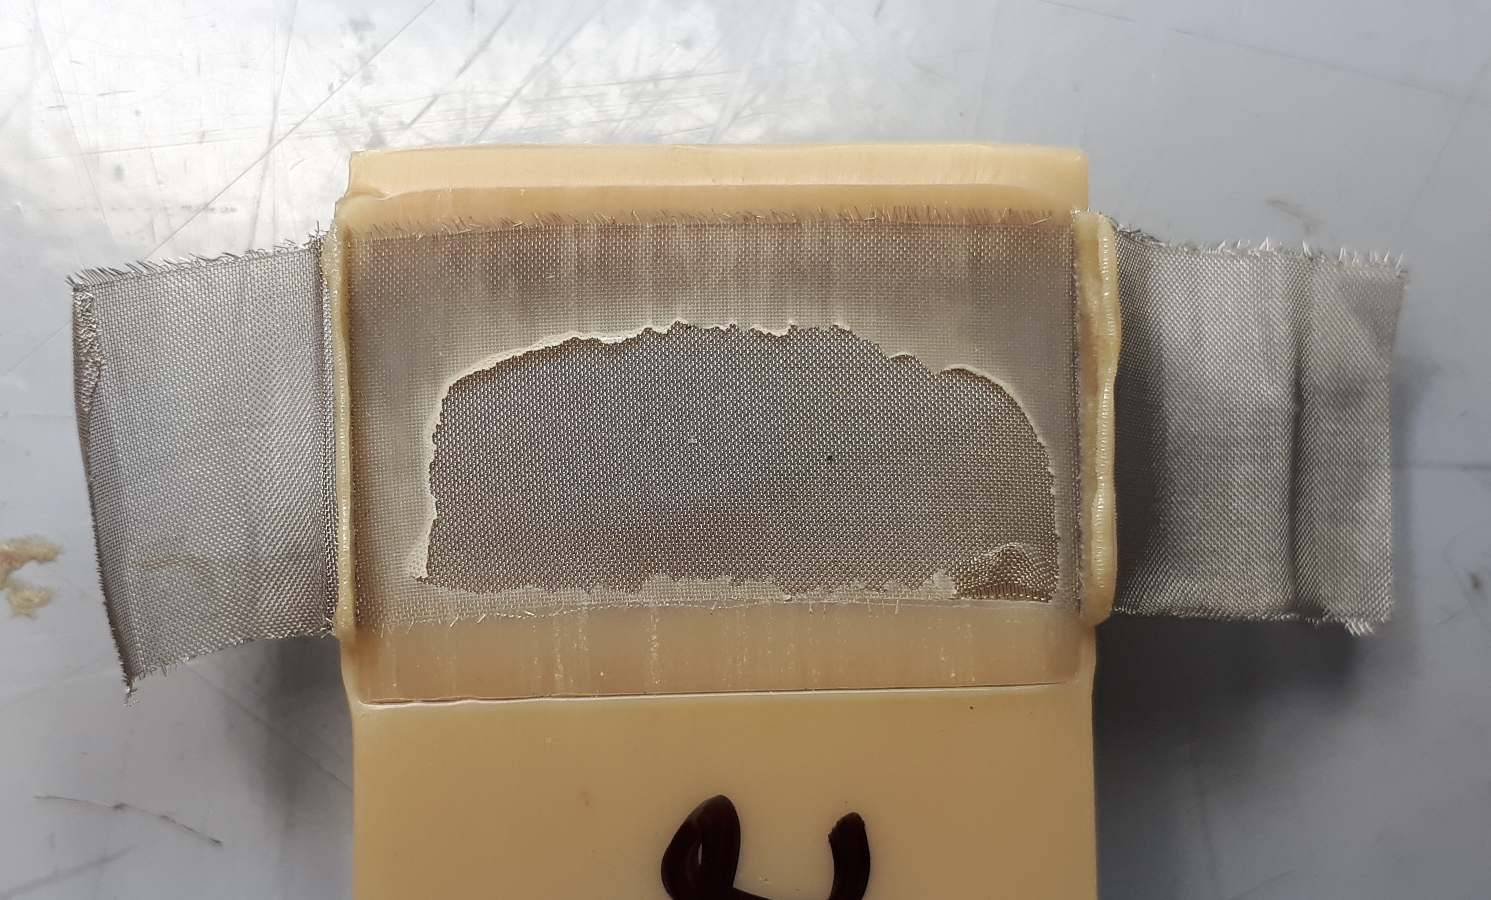
\includegraphics[height=4.25cm]{20190918_112850_crop_resize.jpg}
	} \qquad
	\subfigure[]
	{\label{fig:STM1500_facies2_soudure_SS}
		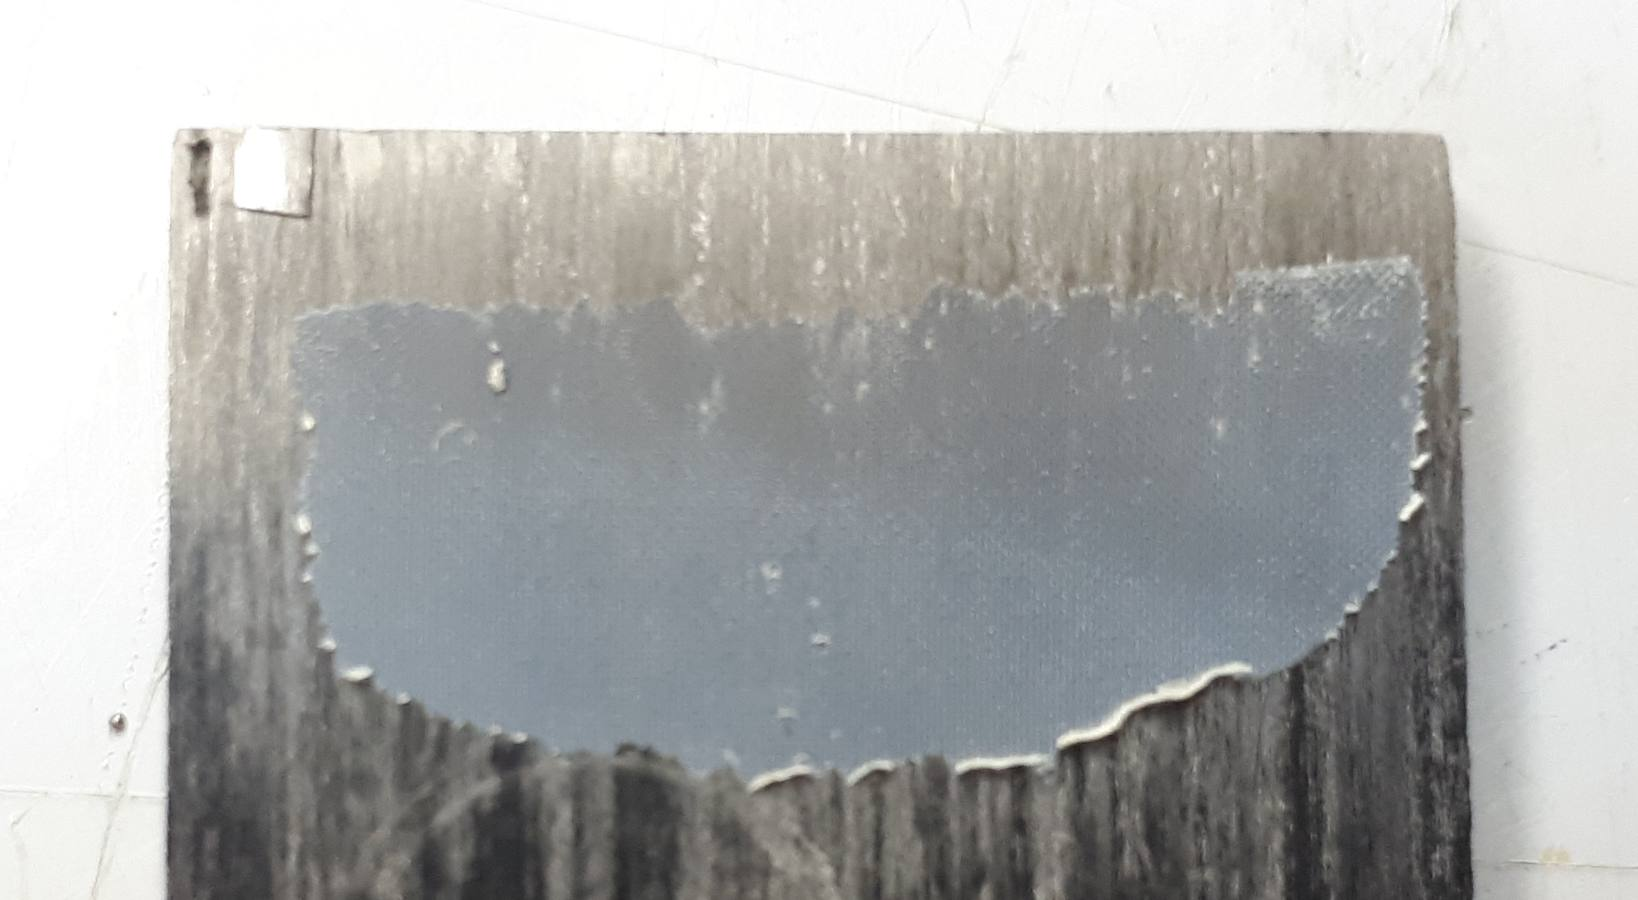
\includegraphics[height=4.25cm]{20190918_112859_crop_resize.jpg}
	}
	\caption{Faciès de rupture à la suite des essais mécaniques pour l'échantillon soudé avec un élément chauffant en acier inoxydable à une puissance de \SI{220}{\kilo\watt\per\square\metre} pendant \SI{45}{\second} présentant a) le côté de l'élastomère et b) le côté du composite}
	\label{fig:STM1500_facies_soudure_SS}
\end{figure}

\FloatBarrier
\subsection{Vérification de la miscibilité du PEI-siloxane}

Un mélange de PEI avec 10\% massique de PEI-siloxane a été produit avec un mélangeur interne. 
Lors de ce mélange, le PEI a été initialement mélangé pendant 10 minutes à \SI[locale=FR]{340}{\celsius} avant d'ajouter l'élastomère et de poursuivre le mélange pendant 3 minutes. 
Le mélange obtenu a été analysé au microscope électronique à balayage afin d'observer la présence ou l'absence de compatibilité et de diffusion entre les phases. 
Les images obtenues (Fig. \ref{fig:SEM_mix_STM1500_PEI}) indiquent que 3 minutes n'ont pas été suffisantes pour obtenir un mélange homogène, puisqu'on dénote deux phases distinctes. 
Cependant, les structures de la section indiquée ont la même morphologie que les structures obtenues lors d'un mélange complet \cite{Hatui2015}. 
L'absence de ségrégation complète, de nodules ou de fissures entre les phases supporte l'idée voulant que 10\% de PEI-siloxane soit miscible dans une matrice de PEI. 
Des essais supplémentaires seront cependant nécessaires pour démontrer hors de tout doute cette miscibilité, puisqu'une simple observation au microscope électronique à balayage ne permet pas d'obtenir des observations à une échelle suffisante pour confirmer le phénomène. 

\begin{figure}[h]
	\centering
	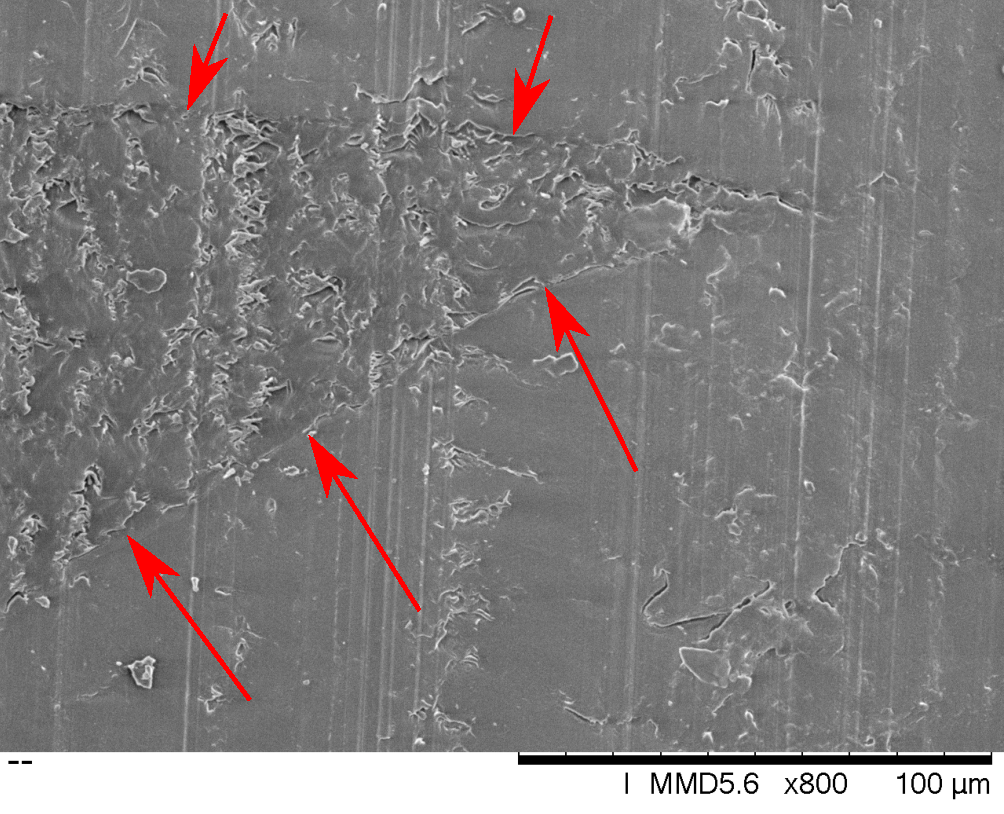
\includegraphics[width=0.7\textwidth]{PEI_STM1500_09(x800).pdf}
	\caption{Observation au microscope électronique à balayage d'un mélange composé de PEI et de 10\% massique de PEI-siloxane}
	\label{fig:SEM_mix_STM1500_PEI}
\end{figure}

\FloatBarrier
\section{Conclusion}

Au vu des résultats obtenus, on peut confirmer que le PEI-siloxane présente le potentiel pour obtenir une jonction soudée. 
Cet élastomère semble miscible dans le PEI jusqu'à une fraction massique supérieure à 10\%. 
Il offre également de bonnes propriétés mécaniques et une excellente stabilité thermique. 
Cependant, jusqu'à présent, il n'a pas été possible de trouver des conditions propices à l'obtention d'une soudure satisfaisante avec une bonne diffusion des chaines de polymères. 
Cet élastomère forme rapidement des porosités lorsqu'il est chauffé et ces dernières empêchent la formation d'une jonction solide. 
Le taux d'humidité dans l'élastomère et le PEI composant le nanocomposite n'ayant pas été pris en compte pour les soudages, il serait approprié d'au moins répéter les essais en laboratoire avec des adhérents et des éléments chauffants ayant été séchés à l'étuve. 
Les porosités rencontrées dans les soudures entre adhérents composites pourraient d'ailleurs être expliquées, en partie, de cette façon. 
Une autre approche qui pourrait être envisagée, à défaut d'une soudure, serait de texturer l'élément chauffant pour améliorer le blocage mécanique entre les phases. 
Un autre point noté durant ces essais est que les cycles thermiques à haute température répétés pour le nanocomposite causent une dégradation de ses propriétés. 
Encore une fois, en raison de la quantité de nanotubes de carbone dans le nanocomposite, la diffusion des chaines de polymères est ralentie et nécessite des températures élevées qui sont propices à la dégradation des polymères. 
Cet effet était visible dans la fenêtre d'opération pour le soudage d'adhérents composites et il a de nouveau un impact pour la production de soudures multimatériaux. 
Les travaux visant à obtenir un soudage multimatériaux n'ont pas permis, pour l'instant, d'aboutir à une solution rencontrant les requis techniques d'ArianeGroup. 